%Review of existing harmonic excitation.
%	Nonlinear Systems
%		Traditional Metrics (THD, IMD)
%		Minimisation of Nonlinear Distortion
%		Advent of "Nonlinear Niceness"
%	Timbre of nonlinear distortions (Martens and Marui type shit)
%	Uses of Harmonic Excitation
%	Harmonic Generation Methods
%		Static Nonlinearities
%		Bandwidth Extension (high frequency reconstruction)
%		Individual Harmonic Generation (SMC paper)
%		Psychoacoustic Enhancers

\chapter{Harmonic Excitation}
\label{chap:Excitation}

\section{Introduction}
\label{sec:Excitation-Introduction}
	Nonlinear distortion is an inherent part of an analogue signal path. It alters the dynamic variation of signals and
	introduces new spectral components. Its use as a creative effect is best know by guitar players
	\citep{dutilleux2011nonlinear}. This was due to the use of values in early guitar amplifiers imparting nonlinear
	transforms onto the audio signal. This distorted sound became desirable and several electronic circuits were
	developed with the purpose of inducing nonlinear distortion. More recently research into modelling these distortion
	circuits in the digital domain has been carried out, such as that done by \citet{pakarinen2009a}. Several
	researchers have also worked on creating novel digital distortion techniques \citep{fernandez-cid2001distortion,
	pekonen2008coefficient, puckette2007patch}.

	Distortion is a very broad term which is typically used to describe unwanted effects. For this work a better defined
	term, harmonic excitation, will be used to refer to the deliberate and controlled application of nonlinear systems
	in order to introduce new frequency components to a signal. \citet{dutilleux2011nonlinear} defines excitation as
	the process of controlling timbre through the emphasis of certain frequencies. While this is possible with linear
	systems, such as equalisers, nonlinear systems provide more flexibility as they can add energy in areas of the
	spectrum where the original signal had none.

	This chapter will review how nonlinear systems have been analysed in previous audio research, how their effects are
	quantified and the timbral transformations they impart. The current uses of harmonic excitation in audio engineering
	are then discussed in Section \ref{sec:Excitation-Uses}. A list of criteria with which to evaluate harmonic
	excitation methods for use in real time timbral control is developed in Section \ref{sec:Excitation-Evaluation}.
	Section \ref{sec:Excitation-Methods} then describes several methods for harmonic excitation and how they perform in
	these areas.  Issues with certain methods are identified and ways to overcome them suggested.

\section{Analysis of Nonlinear Systems}
\label{sec:Excitation-AnalysisOfNonlinearSystems}
	The analysis of nonlinear system is more complicated that that of linear systems. This is due to more features of
	the input signal affecting how the system responds. In the field of audio engineering much of the literature
	concerning nonlinearities has to do with minimising distortion or measuring the maximum allowable levels of
	distortion. Several distortion metrics have been developed each with there own uses. A review of many of these
	metrics is given by \cite{voishvillo2006assessment}, some of which will be discussed in this section.

	\subsection{Objective Distortion Metrics}
	\label{sec:Excitation-Analysis-Metrics}
		Total Harmonic Distortion (THD) and Intermodulation Distortion (IMD) are the traditional objective measures
		of distortion \citep{czerwinski2001multitone1}. THD measures the level of new frequency components
		introduced by a system which are harmonically related to the original signal.  There are two different ways
		in which THD is calculated. These have been denoted $THD_{F}$ and $THD_{R}$ by \citet{shmilovitz2005on} and
		are calculated using Equations \ref{eq:thdf} and \ref{eq:thdr} respectively.

		\begin{equation}
			THD_{F} = \frac{\sqrt{\sum_{n = 2}^{\infty} A_{n}^{2}}}{A_{1}}
			\label{eq:thdf}
		\end{equation}

		\begin{equation}
			THD_{R} = \sqrt{\frac{\sum_{n = 2}^{\infty} A_{n}^{2}}{\sum_{n = 1}^{\infty} A_{n}^{2}}}
			\label{eq:thdr}
		\end{equation}

		Where $A_n$ is the amplitude of the $n_{th}$ harmonic. 

		Both these methods been used in recent work published in the audio field ($THD_{F}$ by
		\citet{fleischmann2014a} and $THD_{R}$ by \citet{dutilleux2011nonlinear}). The lack of standardisation for
		this metric makes it difficult to compare experiment results reported by different sources.

		IMD is a measure of the new spectral content introduced by a system as a result of intermodulation between
		the frequency components of the original signal. There are several different standards for the calculation
		of IMD some of which are listed by \citet{voishvillo2006assessment}.

		THD and IMD give very limited information about the response of nonlinear systems. They are typically
		measured using simple input signals which are not representative of the signals a system would process in
		actual use. Given that nonlinear systems my not satisfy the condition of superposition a system may process
		simple and complex signals in vastly differing manners. 

		These metrics also give no indication of the perceived degradation in audio quality a system introduces. A
		signal with a high THD values may sound less distorted that one with a small THD. Several researchers have
		developed new distortion metrics which indicate the perceived amount of distortion.

		\citet{geddes2003auditory} suggest some psychoacoustic principles which may be applicable to the analysis of
		nonlinear distortion:

		\begin{itemize}
			\item New frequency components introduced, with lower frequencies that the original components, will
			      be more perceptible.
			\item Higher order nonlinearity artefacts will be more perceptible.
			\item Nonlinearities which affect lower amplitude signals will be more perceptible.
		\end{itemize}

		\citet{voishvillo2006assessment} adds that the perception of distortion is decreased at the very high and
		low ends of the frequency spectrum.

		The GedLee metric, proposed by \citet{geddes2003auditory}, measures how much a nonlinearity will be
		perceived through analysis of its characteristic curve. It is calculated using Equation \ref{eq:gedlee}.

		\begin{equation}
			G_{m} = \sqrt{\int_{-1}^{1} \left( \cos \left( \frac{x\pi}{2} \right) \right)^{2}
				      \left( \frac{d^{2}}{dx^{2}} T(x) \right)^{2} dx}
			\label{eq:gedlee}
		\end{equation}

		Where $T(x)$ is the characteristic curve of the nonlinearity in question.

		A considerable advantage of the GedLee metric is that it directly measures the system in question rather
		than signals processed by it. This should allow measurements taken using the metric to describe the audible
		degradation of any signal processed by a system. \citet{lee2003auditory} provide results of an experiment
		in which their metric was tested against THD and IMD as a rating of audio quality. They show that for low
		levels of distortion the GedLee metric correlates with subjective audio quality ratings. THD and IMD are
		both found to not correlate well with perceived quality.

		In Equation \ref{eq:gedlee} the system being analysed is assumed to be a simple static nonlinearity. Many
		nonlinear systems are more complex than this and may exhibit frequency dependant or time varying behaviour.
		While the GedLee metric may provide a good, signal independent, measure of distortion, it is only
		applicable to a subset of nonlinear systems.

		\citet{tan2003the} also developed a perceptual metric for distortion, Distortion Score (DS), which they
		then improved upon to create the R\sub{nonlin} metric \citep{tan2004predicting}. Both these metrics rely on
		analysing signals which have been processed so they may not give results which can be applied as generally
		as those using the GedLee metric. Where these metrics have an advantage is that they use models of the
		human hearing system to better approximate the perceived level of distortion.

		To calculate the DS the audio is split into frequency bands which model the auditory filters of the
		cochlear. These auditory filters represent bands in which two tones will interfere with the perception of
		each other \citep{fastl2007psychoacoustics}. Tones can be masked (made inaudible) by other tones within the
		same auditory filter band. By processing the audio in this manner the DS metric can take account of
		elements of the distortion which may not be perceptible because of masking.
		
		The R\sub{nonlin} metric improves on this model of the hearing system by including a filter with a
		frequency response similar to that of the outer and middle ear. The filter used is as described by
		\citet{glasberg2002a}, it attenuates frequencies at either end of the audible spectrum. This models the
		decreased perception of distortion at these frequencies discussed earlier.

		\citet{tan2004predicting} report greater correlation between R\sub{nonlin} and perceived audio quality then
		\citet{lee2003auditory} do for the GedLee metric. They also demonstrate how accurate the R\sub{nonlin}
		metric is in predicting the perceived distortion level introduced to music and speech signals.

		The research discussed in this section has focused on measuring the extent to which unwanted distortion can
		be perceived. This does not provide enough information for the description of timbre. The listening test
		performed to verify the developed metrics asked subjects to rate the quality of audio samples. Nonlinear
		distortion could alter the timbre of audio without deteriorating its perceived quality. It may also be
		possible to describe the timbre of different nonlinear distortions further rather than ranking them on the
		same distortion scale. Research has been carried out into the timbre of distortion as discussed in Section
		\ref{sec:Excitation-Timbre}.

		\subsection{Nonlinear Modelling}
		Various techniques for modelling nonlinear systems have been developed in the mathematics and engineering
		literature. These models allow for more in depth analysis of a system as well as replicating its effects in
		the digital domain. Summaries of some of these modelling techniques can be found in the work by
		\citet{janczak2005identification} and \citet{ogunfunmi2007adaptive}.

		Two nonlinear modelling techniques have found use in audio processing:

		\begin{itemize}
			\item Wave Digital Filters as discussed by \citet{fettweis1986wave}.
			\item The Synchronised Swept Sine Method as described by \citet{novak2010nonlinear}.
		\end{itemize}

		These techniques are summarised here.

		\subsubsection{Wave Digital Filters}
			Wave digital filters are a class of filter which can be used to emulate analogue circuits. The
			process of creating a digital of a circuit involves constructing a `tree' of blocks. These blocks
			represent either electronic components, or connections between components in a circuit. Each block
			obeys a certain set of rules when presented with a signal. Blocks have been developed for modelling
			nonlinear circuit elements such as operational amplifiers and diodes \citep{paiva2012emulation}.

			While wave digital filters can accurately represent a nonlinear system there are some disadvantages.
			As systems get more complex traversing the `tree' of blocks in order to calculate the output signal
			takes more computation. This presents problems when real time system response is needed. There are
			also certain circuit topologies which cannot be represented in the wave digital domain
			\citep{valimaki2011virtual}. Another consideration is that knowledge of the circuitry inside a
			system being modelled is needed. This might not always be available.

		\subsubsection{The Synchronised Swept Sine Method}
			The synchronised swept sine method is a technique for identifying nonlinear systems without prior
			knowledge of their operation. The details of its operation are describe by
			\citet{novak2010nonlinear}. The result of the testing is a series of filter kernels to be used in
			the model shown in Figure \ref{fig:hammerstein}.

			\begin{figure}[h!]
				\centering
				\begin{tikzpicture}
					\node (Sig2) [draw] at (1, 3) {$x[n]^{2}$};
					\node (Sig3) [draw] at (1, 2) {$x[n]^{3}$};
					\node (SigN) [draw] at (1, 0.5) {$x[n]^{N}$};

					\node (Filter1) [draw] at (3, 4) {$A_{1}(f)$};
					\node (Filter2) [draw] at (3, 3) {$A_{2}(f)$};
					\node (Filter3) [draw] at (3, 2) {$A_{3}(f)$};
					\node (FilterN) [draw] at (3, 0.5) {$A_{N}(f)$};

					\draw (Sig2) -- (Filter2);
					\draw (Sig3) -- (Filter3);
					\draw (SigN) -- (FilterN);

					\draw [dots] (Sig3) -- (SigN);
					\draw [dots] (Filter3) -- (FilterN);

					\coordinate (Out1) at (4.5, 4);
					\coordinate (Out2) at (4.5, 3);
					\coordinate (Out3) at (4.5, 2);
					\coordinate (OutN) at (4.5, 0.5);

					\draw (Filter1) -- (Out1);
					\draw (Filter2) -- (Out2);
					\draw (Filter3) -- (Out3);
					\draw (FilterN) -- (OutN);

					\node (Add) [operator] at (5, 2.25) {+};
					\draw (Out1) -- (Add);
					\draw (Out2) -- (Add);
					\draw (Out3) -- (Add);
					\draw (OutN) -- (Add);

					\coordinate (In1) at (-0.5, 4);
					\coordinate (In2) at (-0.5, 3);
					\coordinate (In3) at (-0.5, 2);
					\coordinate (InN) at (-0.5, 0.5);

					\draw (In1) -- (Filter1);
					\draw (In2) -- (Sig2);
					\draw (In3) -- (Sig3);
					\draw (InN) -- (SigN);
					\draw (InN) -- (In1);

					\node (In) at (-1.25, 2.25) {$x[n]$};
					\coordinate (InMid) at (-0.5, 2.25);
					\draw (In) -- (InMid);

					\node (Out) at (6, 2.25) {$y[n]$};
					\draw (Add) -- (Out);

				\end{tikzpicture}
				\caption{Generalised Polynomial Hammerstein Model.}
				\label{fig:hammerstein}
			\end{figure}

			The model is, in effect, an extension of a Taylor Series of order $N$. The input is raised to each
			individual power, 1 through $N$, and each of these signals is filtered by an individual kernel,
			$A_{N}(f)$. The resultant signals are then summed to produce the output.

			This method is easier to implement that a wave digital filter as no prior knowledge of the system is
			needed. The amount of computation time needed to process a signal is also considerably less. There
			are however some disadvantages. There is no account for the dependence of the system on the
			amplitude of the input signal. This is shown by \citet{novak2010analysis} who demonstrate how two
			different circuits are emulated with different degrees of accuracy. The is also no definite way of
			deciding what order Hammerstein model to use prior to testing.

\section{Timbre of Nonlinear Distortion}
\label{sec:Excitation-Timbre}
	There is a wealth of research into how low level audio features influence timbre \note{(probably refer to stuff in
	the timbre chapter here)}. The mappings between low level features and semantic features from the literature can be
	applied to harmonic excitation effects provided the excitation method used can influence the required low level
	features. There may be semantic terms used to describe the timbre of nonlinear distortion which are seldom used to
	describe other timbres. The majority of timbral research does not focus on nonlinear distortion and as such does not
	highlight these semantic terms. There have been some publications specifically discussing the timbral effects of
	nonlinear distortion. Their findings are discussed in this section.

	\citet{marui2005predicting} suggest that one of the primary outcomes of nonlinear distortion is the moving
	of spectral energy between low and high frequencies. An effect they propose correlates with the descriptors
	sharpness and brightness. In order to discover other timbral properties of nonlinear distortion they performed
	listening tests in which distorted guitar samples were assessed. The samples were each processed with different
	nonlinear systems and then further processed so that they had matching Zwicker Sharpnesses (an objective measure of
	sharpness \cite{fastl2007psychoacoustics}). This sharpness matching was does so that difference in timbre not
	related to sharpness could be more easily observed. During the listening tests subjects were asked to rate the
	dissimilarity of samples presented in pairs. They were also asked to grade each individual sample on the bipolar
	adjective scales shown in Table \ref{tab:distortiondescriptors}.

	\begin{table}[h!]
		\centering
		\begin{tabular}{|c|C{3cm}cC{3cm}|}
			\hline
			\bf{No.} & \multicolumn{3}{|c|}{\bf{Adjectives}} \tabularnewline
			\hline
			\hline
			1 & dark & $\Longleftrightarrow$ & bright \tabularnewline
			\hline
			2 & rough & $\Longleftrightarrow$ & smooth \tabularnewline
			\hline
			3 & diffuse & $\Longleftrightarrow$ & compact \tabularnewline
			\hline
			4 & thin & $\Longleftrightarrow$ & thick \tabularnewline
			\hline
			5 & sharp & $\Longleftrightarrow$ & dull \tabularnewline
			\hline
			6 & light & $\Longleftrightarrow$ & heavy \tabularnewline
			\hline
			7 & hard & $\Longleftrightarrow$ & soft \tabularnewline
			\hline
			8 & clear & $\Longleftrightarrow$ & muddy \tabularnewline
			\hline
			9 & clamorous & $\Longleftrightarrow$ & calm \tabularnewline
			\hline
			10 & string & $\Longleftrightarrow$ & weak \tabularnewline
			\hline
			11 & uncomfortably loud & $\Longleftrightarrow$ & comfortable \tabularnewline
			\hline
		\end{tabular}
		\caption{Bipolar adjectives scales used by \citet{marui2005predicting} to assess the perception of
		         distortion.}
		\label{tab:distortiondescriptors}
	\end{table}

	Their results suggest that the differences between different nonlinearities can be described by `thickness' and, to
	a lesser extent, `diffuseness'. These results are also met by a second experiment in which a triadic comparison
	method is used to assess the dissimilarities between samples \citep{marui2005constructing}.

	Both these experiments were conducted in Japanese and the descriptors were translated to English for publication.
	The descriptors were initially chosen during an experiment by \citet{martens2002relating}. From this experiment it
	was shown that speakers of Japanese and speakers of Sinhalese disagree on the how these terms are used to describe
	timbre. It is expected that there will be similar differences in presenting the descriptors to English speakers.

\section{Uses of Harmonic Excitation}
\label{sec:Excitation-Uses}
	Harmonic excitation is used for several tasks in audio engineering:

	\begin{itemize}
		\item As a creative audio effect used to manipulate the timbre of sounds for music production.
		\item To reconstruct high frequency information in perceptual audio compression codecs.
		\item To extend the perceived bandwidth of loudspeakers.
		\item To enhance the intelligibility of speech. 
	\end{itemize}

	\subsection{High Frequency Reconstruction}
	\label{sec:Excitation-Uses-Reconstruction}
		In digital systems it can be beneficial to reduce the amount of data needed to represent an audio signal.
		This is done either to reduce the storage space needed or reduce the data rate required to transmit a
		signal. As a higher data rate is needed to represent high frequencies these frequencies are removed during
		the compression process. A lot of research has been carried out to develop methods by which these high
		frequencies can be estimated during the decoding process. This allows for the bandwidth to be constricted
		for storage or transmission but the full bandwidth to be restored when required.

		When using audio codecs the original signal, along with is high frequency components, is available before
		compression is applied. This means that some parameters relating to the high frequency content can be
		recorded and used to aid in the reconstruction of the high frequencies later \citep{dietz2002spectral,
		friedrich2007spectral}. The high frequency content is estimated from the low frequency information and
		then further shaped using these parameters. This leads to a distinction between `blind' and `non blind'
		methods for reconstructing the high frequencies. A `blind' method uses only the information present in the
		low frequency signal, whereas `non blind' methods make use of recorded parameters to increase the accuracy
		of the reconstruction.

		In the literature several different methods for reconstruction of the higher frequencies are suggested:

		\begin{itemize}
			\item Through the use of a nonlinear device \citep{larsen2002efficient, sha2010high}.
			\item Spectral replication as done by \citet{nagel2010a}. This essential frequency shift the
			      spectrum into a higher band.
			\item Spectral folding as used by \citet{friedrich2007spectral}. This creates a mirror image of the
			      existing spectrum around the highest frequency.
			\item Spectral stretching a used by \citet{nagel2009a}. This stretches the existing spectrum to the
		              desired bandwidth.
		\end{itemize}

		These methods could be utilised in creative audio effects. They all introduce new harmonic spectral
		components which may enhance perceptual attributes of a sound. In this situation there is not any
		information about how the higher harmonics might behave so the system will have to operate `blindly'. It is
		worth considering that when using these methods as an audio effect the objective is not to try and
		replicate high frequency content which is missing. The generation of new, high order, harmonics does not
		require the same degree of accuracy. The accuracy lost through using `blind' bandwidth extension methods is
		not a great concern for creative timbral manipulation work.

		Information on how these methods can be implemented as simple harmonic exciters is given in Section
		\ref{sec:Excitation-Methods}.

	\subsection{Perceptual Low Frequency Reinforcement}
	\label{sec:Excitation-Uses-Reinforcement}
		Small loudspeakers are incapable of reproducing low frequency signals at sufficient amplitudes. Harmonic
		excitation can be used to psychoacoustically extend the bandwidth of loudspeakers into the lower end of the
		spectrum. Harmonic content is added to the signal in order to evoke the perception of lower pitch sounds.

		The pitch of harmonically structured sounds is the same as that of it's fundamental frequency. No energy
		need be present at the fundamental for its pitch to be perceived however. So long as a sufficient
		proportion of the harmonic structure remains the original pitch can still be perceived. This phenomenon is
		commonly referred to as the missing fundamental \citep{plack2005the}.

		This technique is implemented in effects such as Waves' MaxxBass \citep{ben-tzur1999the}. Implementation
		techniques have been discussed by \citet{larsen2002reproducing} and \citet{gan2001virtual}.

	\subsection{Audio Enhancement}
	\label{sec:Excitation-Uses-Enhancement}
		One of the most commonly used enhancement effects is the Aphex Aural Exciter.  \citet{shekar2013modeling}
		states that this effect enhances brightness and clarity of a sound through the application of nonlinear
		distortion.

		\citet{chalupper2000aural} ran several tests to determine the effects the Aural Exciter has on different
		audio samples, concluding that it operates as a `sharpness' maximiser. The analysis of the device is very
		basic, comprising of a frequency response and an analysis of the spectral alterations made to a 2kHz sine
		wave. The frequency response shows the liner processing undertaken by the device, showing that it amplifies
		high frequency content. The sine wave response analysis is used to demonstrate the nonlinear elements of the
		device. 

		\citet{dutilleux2011nonlinear} provides a slightly more in depth analysis of the Aural Exciter showing the
		spectral alterations make to a chirp signal. This gives information about how the nonlinear section of the
		device responds to different input frequencies. It is seen that a hight level of second harmonic distortion
		is produced. It is not mentioned however, what the exciter's parameters were set to during these tests. For
		this reason it is difficult to compare these results with those collected by \citet{chalupper2000aural}
		which see to disagree as they show a larger amount of new spectral content being introduced. Neither work
		accounts for differences in processing depending on the input amplitude.

\section{Evaluation Criteria for Harmonic Excitation Methods} % section name not very clear
\label{sec:Excitation-Evaluation}
	There are many different classes of nonlinear system which are used in audio processing. Each of these has its own
	characteristics. There are several properties to look at when evaluating a nonlinear system for use in real time
	timbral control. These are:

	\begin{itemize}
		\item Low Complexity.
		\item Homogeneity
		\item Spectral Characteristics.
		\item Temporal Characteristics.
		\item Flexibility.
%		\item Naturalness.
	\end{itemize}

	The following sections will discuss what behaviour is desirable in these areas.

	\subsection{Complexity}
	\label{sec:Excitation-Evaluation-Complexity}
		Audio effects are typically required to operate in real time. This speeds up music production as effect
		parameters can be adjusted while audio is playing and the results heard immediately. In order to achieve
		this, effects must process audio with minimal latency. 

		In order to ease the computational load on the processor, audio processing if often done in blocks. A
		certain number of samples are recorded into a buffer and then all processed at once. This introduces some
		latency into the system, one buffers worth of samples must be collected from the input before an output can
		be produced. The larger the processing buffer size the more latency but the less the computational load. Any
		processing applied to the block of audio must be completed within the allowed latency time. If not there
		will be gaps between blocks during playback causing audible anomalies.

		For real time audio effects it is crucial to keep throughput latency to a minimum. \citet{lester2007the}
		suggest that, depending on the scenario, latencies as small as 1.4ms could be deemed unacceptable. In order
		to keep latency to a minimum, processing algorithms should be able to run in real time when using a small
		buffer size.

	\subsection{Homogeneity}
	\label{sec:Excitation-Evaluation-Homogeneity}
		In order to aid in the intuitiveness of an audio effect it should produce a similar perceptual effect
		across a wide range of input signals. This is not the case with traditional audio signal processing
		methods. Take the EQ for example. We can set up an EQ to boost some frequencies in a desired range. A
		problem arises where we process signals which have no energy in this frequency range. For some signals
		there will be a noticeable change in the spectral characteristics, but other signals will remain unchanged.

		This problem is compounded when the effect being applied is non-homogeneous. A homogeneous system is one
		whose behaviour does not depend on the input amplitude of the input. Where $f$ is a homogeneous system we
		have:

		\[ f(ax) = af(x) \]

		Where $a$ is some scaling factor of the input $x$.
		
		Nonlinear systems are typically non-homogeneous. This is undesirable when using them to achieve timbral
		control as it means the effects are less easy to predict. Different timbral transformations could be
		applied to the same signal if its amplitude is changed slightly. From a user point of view this makes
		control of the system less intuitive as control parameters can change function depending on signal level.

		\note{Mention of homogeneous nonlinear systems \citep{larsen2004audio}.}

		There do exist homogeneous nonlinear systems. These are a minority however and lack some of the desirable
		features that some non-homogeneous systems have. In some cases steps can be taken to make non-homogeneous
		systems homogeneous. These will be discussed where appropriate in Section \ref{sec:Excitation-Methods}

	\subsection{Spectral Characteristics}
	\label{sec:Excitation-Evaluation-SpectralCharacteristics}
		All the systems discussed in this chapter introduce new spectral content to a signal. For timbral control
		it is desirable to have precise control over which frequencies are introduced. Some algorithms introduce
		large bands of frequencies whereas others can be used to excite single harmonics. 
		
		This content can be ascribed to three different groups:

		\begin{itemize}
			\item Harmonic Distortion
			\item Intermodulation Distortion
			\item Aliasing
		\end{itemize}

		These groups are all produced via different mechanisms. 

		\subsubsection*{Harmonic Distortion}
			Harmonic distortion typically refers to the harmonic frequency content generated when a sinusoidal
			signal undergoes nonlinear processing. These are equivalent to the cross modulation components
			introduced by modulating the signal with itself. This mechanism also operates on more complex
			signals. Each individual frequency component being modulated by itself and generating its own set
			of harmonics.

			The spectral effects of harmonic distortion are easy to predict. The response of a system to a
			sinusoidal input can be measured. Then, taking into account any frequency dependence the system may
			have, a general model of how the system will respond to a sinusoid of any frequency can be
			constructed.

		\subsubsection*{Intermodulation Distortion}
			Intermodulation distortion occurs when signals with two or more frequency components undergo
			nonlinear processing. New frequency components are generated equivalent to the cross modulation
			components of each combination of frequency components modulating each other. The more complex the
			spectrum of a signal the more intermodulation components will be introduced. Unlike with harmonic
			distortion it is difficult to generalise the intermodulation components produced by a system. 

		\subsubsection*{Aliasing}
			Aliasing arises due to the discrete nature of digital audio signals. The sampling frequency of a
			discrete signal imposes a restriction on the highest frequency which can be represented. This
			frequency is known as the Nyquist frequency ($f_{N}$) and can be calculated using Equation
			\ref{eq:nyquist}.

			\begin{equation}
				f_{N} = \frac{f_{s}}{2}
				\label{eq:nyquist}
			\end{equation}

			Where $f_{s}$ is the sampling rate of the signal.

			When sampling a signal frequency content above the Nyquist is represented as alias frequencies
			within the bandwidth allowed by the sampling frequency. The alias frequency can be calculated using
			Equation \ref{eq:aliasing}.

			\begin{equation}
				f_{alias} = |f - Nf_{s}|
				\label{eq:aliasing}
			\end{equation}

			Where $f$ is the original frequency and $Nf_{s}$ is the integer multiple of the sampling
			frequency closest to it.

			The new frequency content introduced to a discrete signal via nonlinear processing is also subject
			to aliasing. This can cause problems in the uniformity of behaviour of a system in different
			scenarios as the spectral content introduced will depend on the sampling frequency of the signal
			being processed. Thus the perceived timbral transformation may also depend on the sampling
			frequency.

			\citep{vetter2013estimation} upsample signals by a factor of 32 prior to applying
			the nonlinearity. Afterwards the signal is downsampled to the original sampling frequency. This
			successfully mitigates aliasing as any aliased frequencies which appear in the audible spectrum
			will most likely be inaudible due to having very low amplitudes. It does however increase the
			computational complexity of the system. Along with the extra overhead of upsampling and
			downsampling the signal, there is also 32 times the amount of samples to process.
			There are two common methods to avoid unwanted aliasing distortion in nonlinear effects:

			For certain excitation methods it may be possible to reduce aliasing by changing properties of the
			processing algorithm. Details of these techniques will be discussed where appropriate in Section
			\ref{sec:Excitation-Methods}.

	\subsection{Temporal Characteristics}
	\label{sec:Excitation-Evaluation-TemporalCharacteristics}
		\citep{larsen2004audio} discuss the temporal effects of several bandwidth extension algorithms. Their
		primary concern however is insuring that as little alteration is made to the temporal envelope of a signal
		as possible. For timbral manipulation it is not necessary to be this restrictive. As discussed in Section
		\ref{sec:Timbre-Features} one of the properties of a signal which contributes to its timbre is how it
		evolves over time. As with other aspects of excitation algorithms it is more important that the temporal
		characteristics are predictable and consistent across a wide range of signals.

	\subsection{Flexibility}
	\label{sec:Excitation-Evaluation-Flexibility}
		Each excitation method allows for different amounts of control over the spectral content introduced. Finer
		control of this allows a method to be used in a wider range of situations. The flexibility of a method
		describes how well it can be adapted for different processing needs and how applicable it is across a wide
		range of input signals.

%	\subsection{Naturalness}
%	\label{sec:Excitation-Evaluation-Naturalness}

\section{Harmonic Generation Methods}
\label{sec:Excitation-Methods}
	Several harmonic excitation algorithms have been proposed in the literature. In the section these algorithms are
	evaluated against the criteria given in Section \ref{sec:Excitation-Evaluation}. Techniques for improving
	performance with regard to particular criteria are suggested and discussed. 

	\subsection{Static Nonlinearities}
	\label{sec:Excitation-Statics}
		Static nonlinearities are simple mappings between input value and output value. A nonlinear function is
		applied individually to each sample of a signal. They can be described by a characteristic curves which
		shows the relationship between input and output values.
		
		A very simple class of static nonlinearities is the peak clipper. This class of effects limits the
		magnitude of samples to being at or below a given clipping threshold value. Peak clippers are typically
		piecewise functions comprising of three sections:

		\begin{enumerate}
			\item A linear section. Applied to low magnitude samples.
			\item A transition section, often called the `knee'. This refers to the nonlinear part of the
				function for samples with magnitude below the clipping threshold.
			\item A clipping section. Limiting the magnitude of samples above the clipping threshold.
		\end{enumerate}

		One of the simplest peak clippers is the symmetric hard clipper shown in Equation
		\ref{eq:SymmetricHardClipping}.

		\begin{equation}
			y[n] = \begin{cases}
				t\sgn(x[n]) & \text{if $|x[n]| > t$} \\
				x[n] & \text{otherwise}
			\end{cases}, \quad t \geq 0
			\label{eq:SymmetricHardClipping}
		\end{equation}

		Where $t$ is the threshold value at which to clip the signal. Peak clippers are described as symmetric if
		the underlying function is odd. Clippers which use non odd functions are referred to as asymmetric.

		Equation \ref{eq:SymmetricHardClipping} describes a hard clipper due to the lack of a transition section.
		Soft clippers apply a nonlinear function to medium magnitude samples in order to smooth the transition
		between linear and clipping sections. Equation \ref{eq:SymmetricSoftClipping} shows a soft clipper adapted
		from one given by \citet{dutilleux2011nonlinear}. Figure \ref{fig:Clipping} shows the characteristic curves
		for the clippers given in Equations \ref{eq:SymmetricHardClipping} and \ref{eq:SymmetricSoftClipping}.

		\begin{equation}
			y[n] = \begin{cases}
				t\sgn(x[n]) & \text{if $|x[n]| > t$} \\
				t\sgn(x[n]) \left( 1 - \frac{4}{3} \left( 1 - \left| \frac{x[n]}{t} \right| \right)^{2}
					\right) & \text{if $\frac{t}{2} \leq |x[n]| \leq t$} \\
				\frac{4x[n]}{3} & \text{otherwise}
			\end{cases}, \quad t \geq 0
			\label{eq:SymmetricSoftClipping}
		\end{equation}

		\begin{figure}[h!]
			\centering
			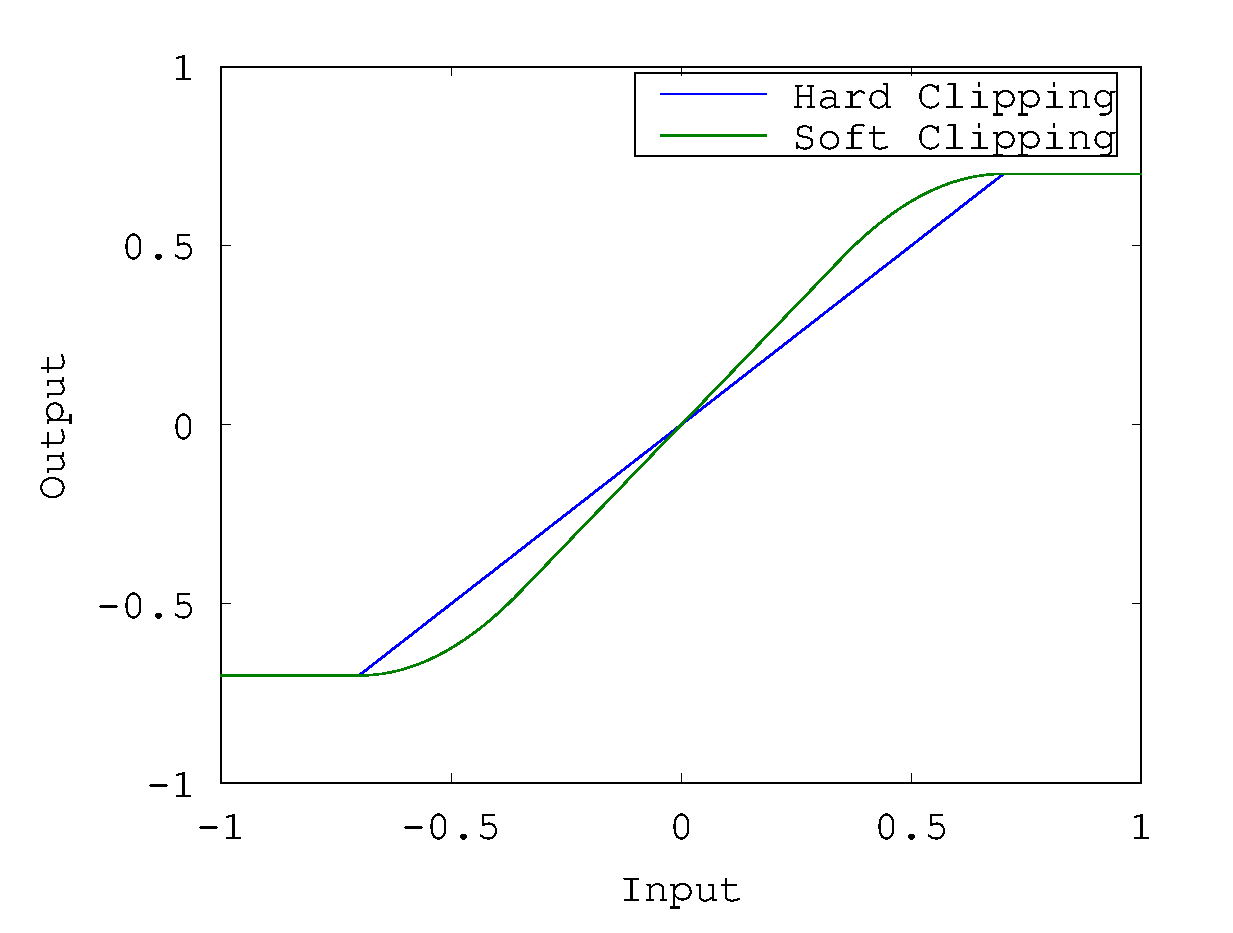
\includegraphics[width=0.6\textwidth]{chapter3/Images/Clipping.eps}
			\caption{Characteristic curves for \ref{eq:SymmetricHardClipping} and
				 \ref{eq:SymmetricSoftClipping} with a threshold of 0.5.}
			\label{fig:Clipping}
		\end{figure}

		\subsubsection*{Complexity}
			Most static nonlinearities only involve a few simple operations for each sample of the input
			signal. The hard clipper from Equation \ref{eq:SymmetricHardClipping} involves only comparisons and
			assignments. A soft clipper could also involve some multiplication and addition.
			
			As each sample is processed individually these algorithms have linear complexity.

		\subsubsection*{Homogeneity}
			The homogeneity of a static nonlinearity depends on the nonlinear function used. For different
			input amplitudes the set of harmonics generated by a given static nonlinearity will change. The
			ways in which this set of harmonics changes was investigated by \citet{enderby2012harmonic}.

			In that study the effects of several soft clippers on sinusoidal inputs were analysed. The levels
			of individual harmonics are plotted as a function of input amplitude. Figures
			\ref{fig:HardClippingHarmonics} and \ref{fig:SoftClippingHarmonics} show these plots for the
			clipping functions described previously.

			\begin{figure}[h!]
				\centering
				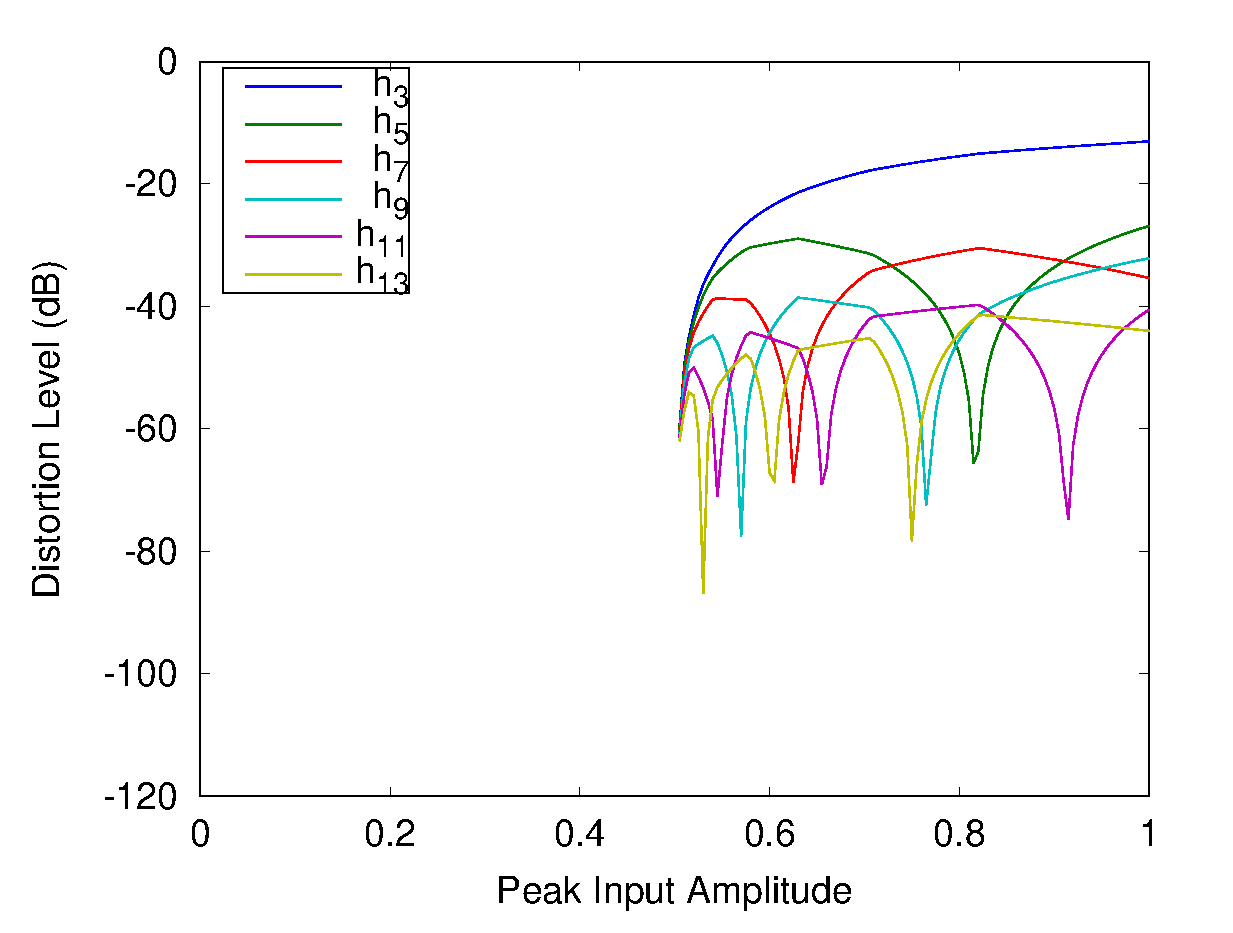
\includegraphics[width=0.6\textwidth]{chapter3/Images/HardClippingHarmonics.eps}
				\caption{Individual harmonic distortion levels for Equation \ref{eq:SymmetricHardClipping}
					 with a threshold of 0.5.}
				\label{fig:HardClippingHarmonics}
			\end{figure}

			\begin{figure}[h!]
				\centering
				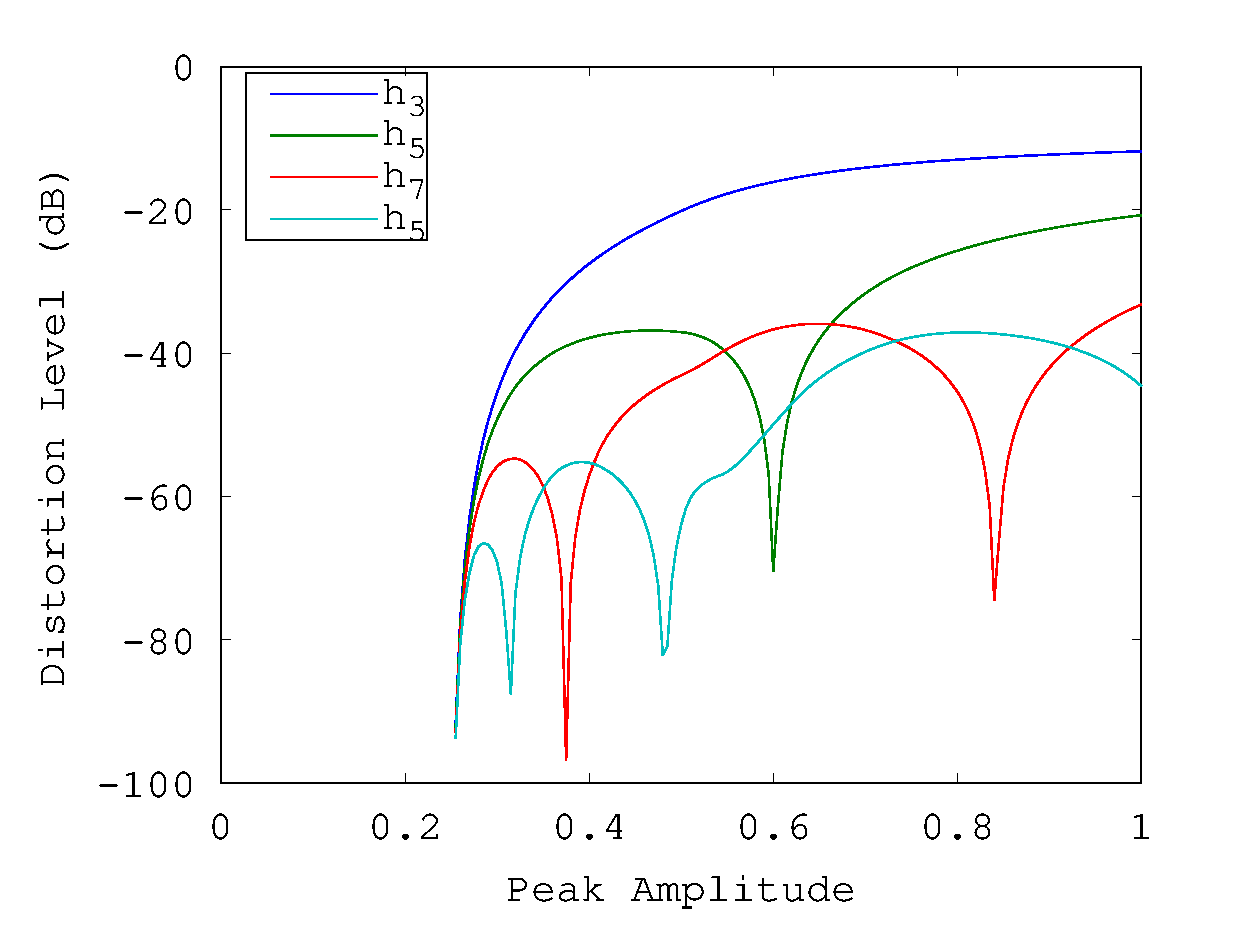
\includegraphics[width=0.6\textwidth]{chapter3/Images/SoftClippingHarmonics.eps}
				\caption{Individual harmonic distortion levels for Equation \ref{eq:SymmetricSoftClipping}
					 with a threshold of 0.5.}
				\label{fig:SoftClippingHarmonics}
			\end{figure}

			The first thing to note is that new harmonic components are only introduced once the input
			amplitude extends out of the linear section of the characteristic curve. Once input amplitude
			reaches a sufficient level harmonics are introduced but their amplitudes all vary independently.

			This behaviour can be improved on through the use of a different clipping function. Equation
			\ref{eq:SymmetricExponentialClipping} shows a function used to apply exponential clipping to a
			signal.
			
			\begin{equation}
				y[n] = \begin{cases}
					t\sgn(x[n]) & \text{if $|x[n]| > t$} \\
					t\sgn(x[n]) \left(1 - \left|\frac{x[n]}{t} - \sgn(x[n]) \right|^{E} \right) &
						\text{otherwise}
				\end{cases}, \quad t \geq 0 \ \text{and} \ E > 1
				\label{eq:SymmetricExponentialClipping}
			\end{equation}

			Where $E$ is a second parameter called the exponent. One advantage of this clipper is that it has
			no linear section. This means that harmonics are generated for input signals of any amplitude.
			Another advantage is that the levels of the generated harmonics vary more uniformly with input
			amplitude as shown in Figure \ref{fig:ExponentialClippingHarmonics}.

			\begin{figure}[h!]
				\centering
				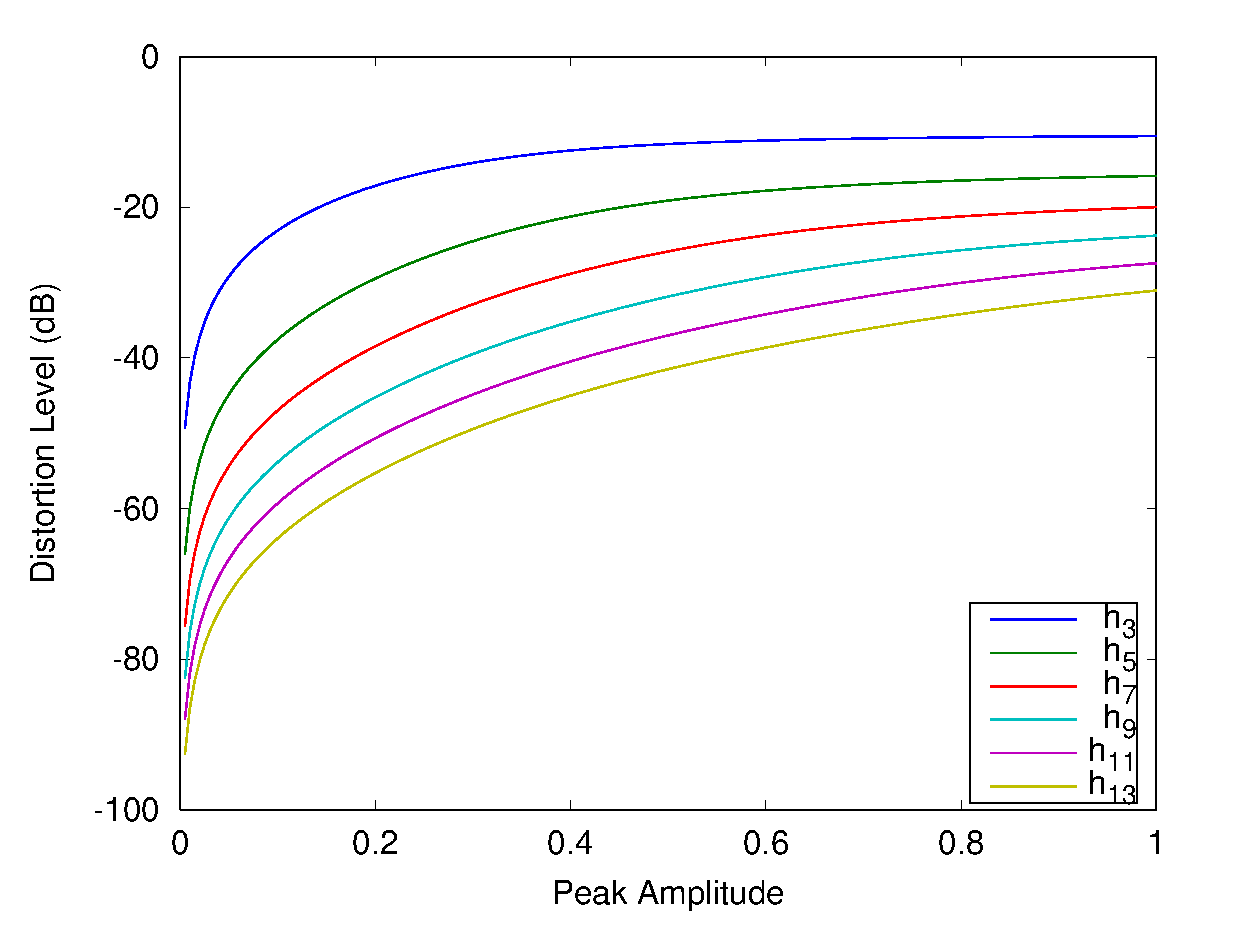
\includegraphics[width=0.6\textwidth]{chapter3/Images/ExponentialClippingHarmonics.eps}
				\caption{Individual harmonic distortion levels for Equation
					 \ref{eq:SymmetricExponentialClipping} with a threshold of 0.5 and an 
				         exponent of 5.}
				\label{fig:ExponentialClippingHarmonics}
			\end{figure}

			The non-homogeneity of simple clipping systems can be counteracted by introducing gain stages
			either side of the clipping stage. The first gain stage scales the signal so that the clipping
			stage will always clip the same proportion of the signal. The second gain stage scales the signal
			back to the original input amplitude. Analogously the clipping function can be scaled so as to
			always clip the same proportion of the signal, as done by \citet{deman2014adaptive}.

		\subsubsection*{Spectral Characteristics}
			The spectral characteristics depend on the function applied to the signal. If an odd function is
			used only odd order components will be produced. Using an even function only even order components
			are generated. 

			The symmetric clippers discussed previously all use odd functions. It is evident from the harmonic
			amplitude plots (Figures \ref{fig:HardClippingHarmonics}, \ref{fig:SoftClippingHarmonics} and
			\ref{fig:ExponentialClippingHarmonics}) that only odd order harmonics have been introduced to the
			signal. In order to generate even order harmonics these clipping function need to be made
			asymmetric. This is easily done by clipping negative and positive portions of the input signal at
			different thresholds. For example, Equation \ref{eq:SymmetricHardClipping} can be modified to allow
			for asymmetric clipping giving Equation \ref{eq:AsymmetricHardClipping}.
			
			\begin{equation}
				y[n] = \begin{cases}
					t_{+} & \text{if $x[n] > t_{+}$} \\
					t_{-} & \text{if $x[n] < t_{-}$} \\
					x[n] & \text{otherwise}
				\end{cases}, \quad t_{-} < t_{+}
				\label{eq:AsymmetricHardClipping}
			\end{equation}

			Where $t_{+}$ and $t_{-}$ are the clipping thresholds for positive and negative portions of the
			signal respectively.	

			Figure \ref{fig:AsymmetricHardClippingHarmonics} show the harmonic amplitude plot for Equation
			\ref{eq:AsymmetricHardClipping} with $t_{+} = 0.5$ and $t_{-} = 0.3$. While the system is still
			non-homogeneous there is a greater amount of new harmonic content.

			\begin{figure}[h!]
				\centering
				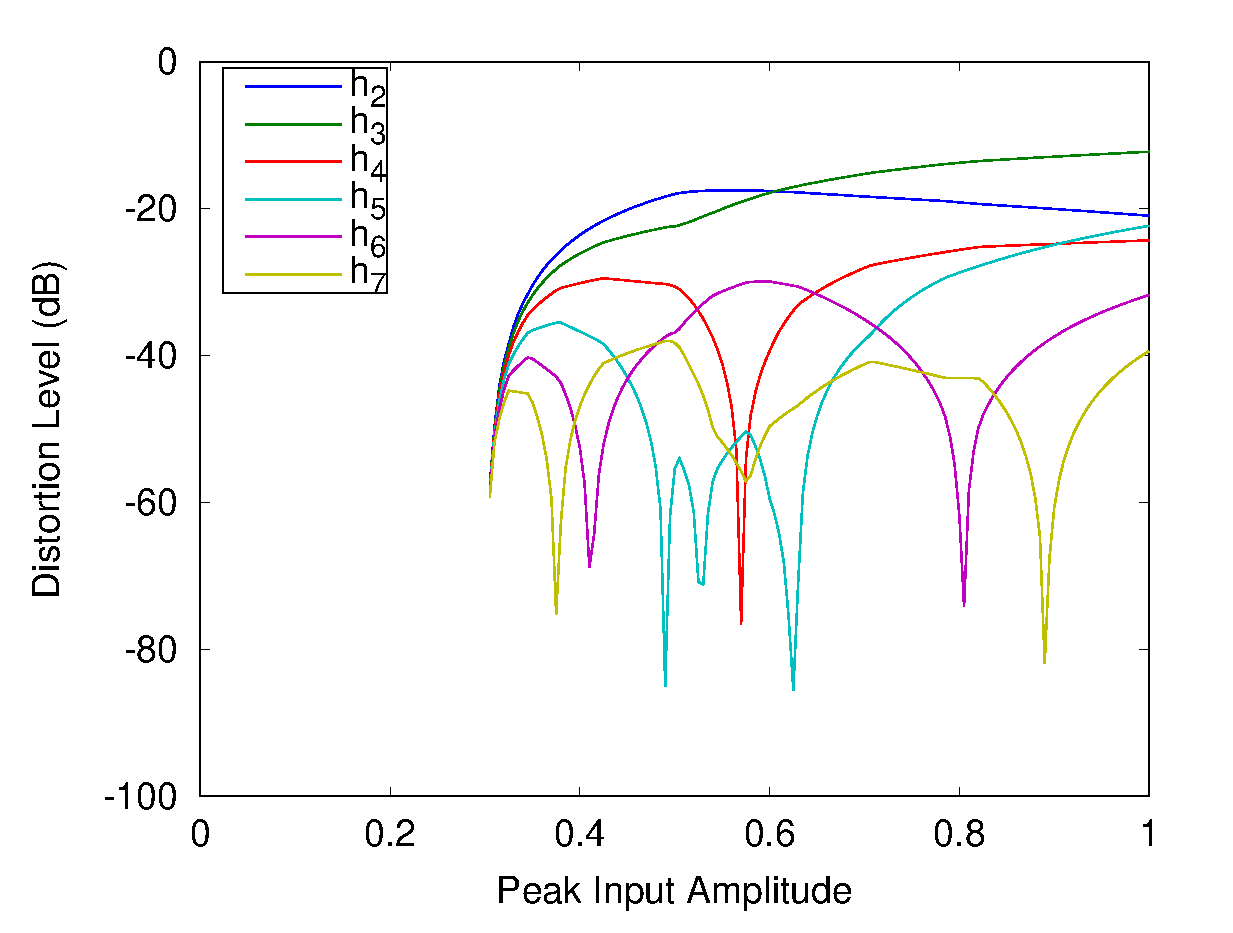
\includegraphics[width=0.6\textwidth]{chapter3/Images/AsymmetricHardClippingHarmonics.eps}
				\caption{Individual harmonic distortion levels for Equation
					 \ref{eq:AsymmetricHardClipping} with thresholds of -0.3 and 0.5.}
				\label{fig:AsymmetricHardClippingHarmonics}
			\end{figure}

			The amplitudes of the generated harmonics will roll off at differing rates depending on the
			properties of the output signal. The spectrum will roll off at $6(n+1)$dB per octave when the
			$n^{\text{th}}$ derivative of the output signal is discontinuous \citep{kraght2000aliasing}.

			Hard clippers introduce discontinuities to the first derivative of a signal and so will introduce
			harmonics whose amplitudes will roll off at 12dB per octave. Signals clipped by Equation
			\ref{eq:SymmetricSoftClipping} are continuous in the first derivative and so produce harmonics
			which roll off at a faster rate. This can be seen in Figure \ref{fig:ClippingSpectra}.

			\begin{figure}[h!]
				\centering
				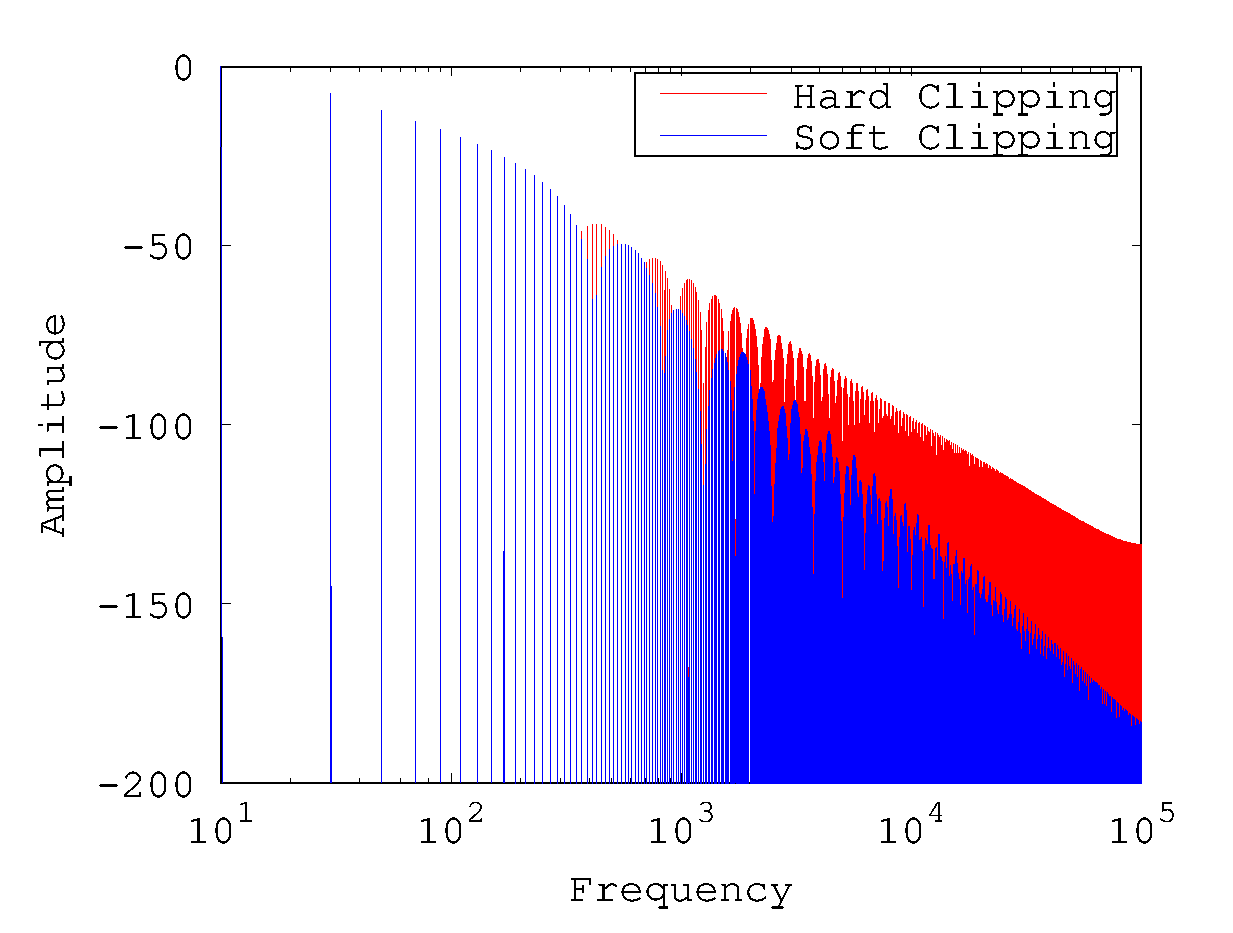
\includegraphics[width=0.6\textwidth]{chapter3/Images/ClippingSpectra.eps}
				\caption{Spectra of sinusoids clipped using Equations \ref{eq:SymmetricHardClipping} and
			                 \ref{eq:SymmetricSoftClipping}.}
				\label{fig:ClippingSpectra}
			\end{figure}

			The large amount of spectral content introduced by static nonlinearities means they are
			particularly susceptible to aliasing. Through smoothing the characteristic curve of the
			nonlinearity (making the clipper `softer') the amplitudes of generated frequencies will roll of
			more quickly. With lower levels of high order distortion the amplitudes of any aliased components
			will be reduced.

		\subsubsection*{Temporal Characteristics}
			As static nonlinearities are memoryless they can not influence the temporal evolution of signals at
			a large scale. There is a possibility to affect the attack and release times of signals slightly
			through increasing the gradient of the low amplitude section characteristic curve. As an extreme
			example consider the infinite peak clipper shown in Equation \ref{eq:InfinitePeakClipper}.

			\begin{equation}
				y[n] = \begin{cases}
					-1 & \text{if $x[n] < 0$} \\
					0 & \text{if $x[n] = 0$} \\
					1 & \text{if $x[n] > 1$}
				\end{cases}
				\label{eq:InfinitePeakClipper}
			\end{equation}
			
			Figure \ref{fig:InfinitePeakClipping} shows a signal, with attack and release sections, before and
			after infinite peak clipping. The original signal rises to it's full amplitude over two cycles and
			falls back to silence over the same time. After infinite peak clipping the attack and release have
			become instantaneous.

			\begin{figure}[h!]
				\centering
				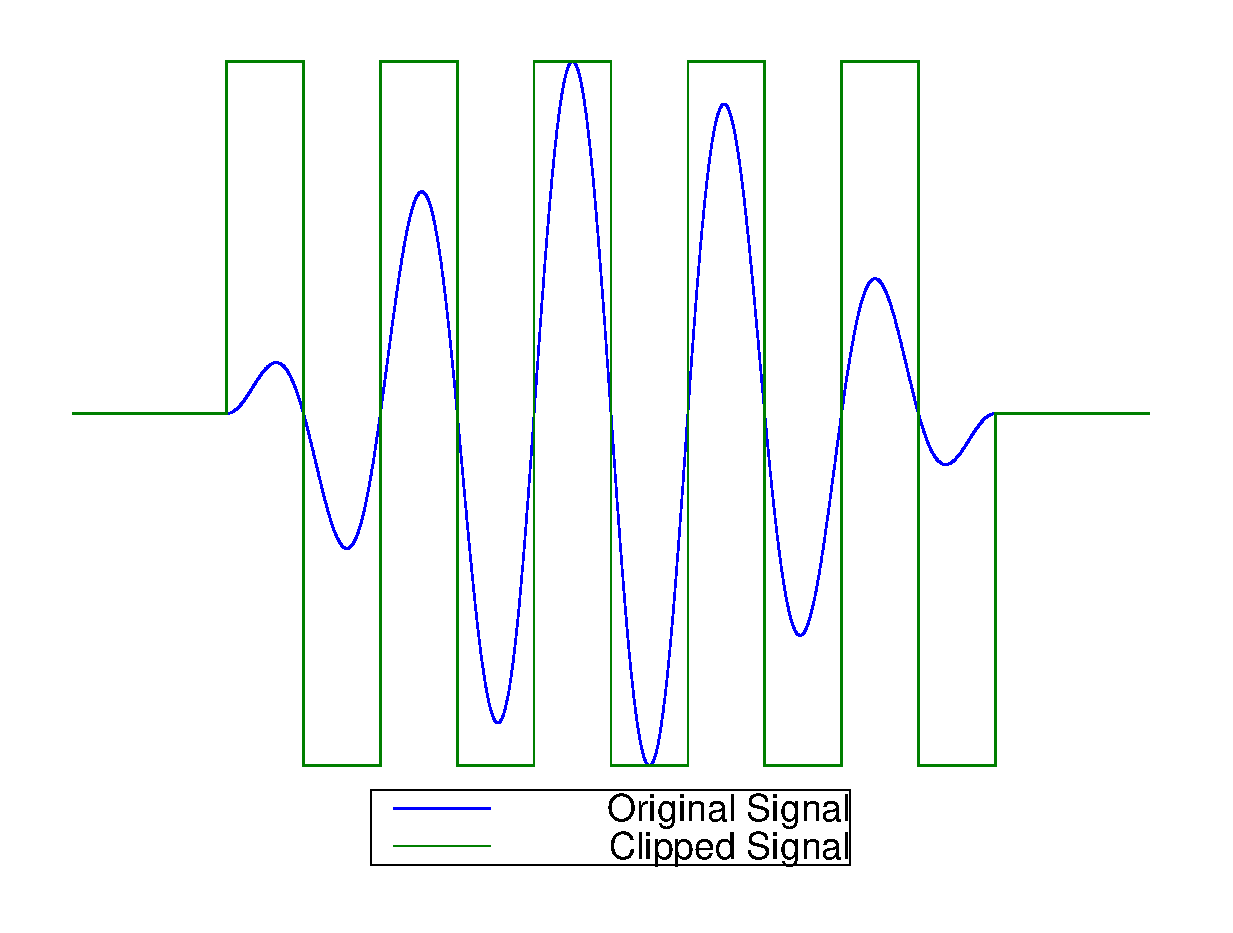
\includegraphics[width=0.6\textwidth]{chapter3/Images/InfinitePeakClipping.eps}
				\caption{A graph showing a signal before and after infinite peak clipping.}
				\label{fig:InfinitePeakClipping}
			\end{figure}

%		\subsubsection*{Flexibility}
%			For musical signals static nonlinearities introduce a spectrally rich band of audio. The spectral
%			content of which is highly dependent on that of the input signal. The bandwidth of the new set of
%			frequencies can be easily controlled through filtering or through the techniques discussed for
%			reducing aliasing. This allows for good performance in situations where energy needs to be added to
%			a specific area of the spectrum. 
			
%		\subsubsection*{Naturalness}

	\subsection{Rectification}
	\label{sec:Excitation-Rectification}
		Rectification is a special case of static nonlinearity. Signals can be either half or full wave rectified,
		as shown in Equations \ref{eq:HalfWaveRectification} and \ref{eq:FullWaveRectification} respectively.

		\begin{equation}
			y[n] = \begin{cases}
				0 & \text{if $x[n] < 0$} \\
				x[n] & \text{otherwise}
			\end{cases}
			\label{eq:HalfWaveRectification}
		\end{equation}

		\begin{equation}
			y[n] = |x[n]|
			\label{eq:FullWaveRectification}
		\end{equation}

		\subsubsection*{Complexity}
			As with other static nonlinearities, rectifiers are very efficient. For full wave rectification
			only a single absolute value operation need be performed on each sample. Half wave rectification
			requires a comparison operation to detect negative samples before an assignment operation is
			applied.

		\subsubsection*{Homogeneity}
			One of the main advantages of rectifiers is that they are homogeneous systems. In half wave
			rectification the magnitude of negative samples is eliminated irrespective of any gain which may
			have been applied to them. In full wave rectification the absolute value of every sample is taken
			preserving their magnitude and thus any gain which has been applied.

		\subsubsection*{Spectral Characteristics}
			Full wave rectification can be considered as a static nonlinearity with an even characteristics
			curve. As such it only introduces even order distortion components. The Fourier coefficients of a
			rectified sine wave are shown in Equation \ref{eq:RectificationFourier}.

			\[ c_{n} = \frac{1}{\pi} \int_{-\pi}^{\pi} |sin(x)|e^{-inx} dx \]

			\[ c_{0} = \frac{2}{\pi} \]
			\begin{equation}
				c_{n} = \begin{cases}
					\frac{2}{\pi(1 - n^{2})} & \text{when $n$ is even} \\
					0 & \text{when $n$ is odd}
				\end{cases}
				\label{eq:RectificationFourier}
			\end{equation}

			This represents all even order harmonics rolling off at approximately 12dB per octave.  As with
			other static nonlinearities rectifiers are susceptible to aliasing. The relatively shallow roll off
			of the distortion components can lead to a considerable amount of energy present in the aliased
			components of the output signal. 

			The output from a half wave rectifier has the same spectrum as that of a full wave rectifier
			but with the content of the original signal included. This can easily be shown by considering how a
			half wave rectified signal can be constructed from the original signal and a full wave rectified
			signal. Where $x(n)$, $x_{f}(n)$ and $x_{h}(n)$ represent the original signal, full wave rectified
			and half waves rectified signals respectively, their relationship can be seen in Equation
			\ref{eq:RectificationRelationship}.

			\begin{equation}
				x_{h}[n] = \frac{1}{2} \left( x_{f}[n] + x[n] \right)
				\label{eq:RectificationRelationship}
			\end{equation}

		\subsubsection*{Temporal Characteristics}
			Full wave rectifiers have no effect on the temporal characteristics of signals as all the magnitude
			of each sample is preserved. It is possible that a half wave rectifier could change the position of
			the onset of a signal by a small amount. Considering a signal which starts with a negative
			displacement. This first section of the signal would be removed, moving the onset to wherever the
			first positive displacement occurs.
			
%		\subsubsection*{Flexibility}
%			Rectifiers are useful when large amounts of even order distortion components are required. As with
%			other static nonlinearities the bandwidth of the newly introduced set of frequencies can be
%			controlled through filtering to provide more flexibility. 

%		\subsubsection*{Naturalness}

	\subsection{Integrator}
	\label{sec:Excitation-Integrator}
		Equation \ref{eq:Integrator} shows an Integrator adapted from the one described by \citet{larsen2004audio}.

		\begin{equation}
			y[n] = \begin{cases}
				0 & \text{if $x[n] > 0$ and $x[n - 1] \leq 0$} \\
				y[n - 1] + k|x[n]| & \text{otherwise}
			\end{cases}
			\label{eq:Integrator}
		\end{equation}

		Where $k$ is the integration constant, effectively setting the output gain of the system. The output signal
		is reset to 0 ofter every negative to positive zero crossing in order to prevent the sample amplitudes from
		rising indefinitely.

		\subsubsection*{Complexity}
			For each sample two comparison operations are required to detect zero crossings. This is followed
			by some simple arithmetic operations in order to integrate the signal. While this may total more
			operations than a very basic static nonlinearity it still requires very little processing power.

			Unlike static nonlinearities the integrator shown in Equation \ref{eq:Integrator} requires memory
			to store the previous output sample. 

		\subsubsection*{Homogeneity}
			Integration is a homogeneous operation. This is an advantage over certain static nonlinearities as
			though more operations are needed per sample no further work is needed to make the system
			homogeneous. If a homogeneous system is required it may be more efficient to use an integrator over
			a static nonlinearity.
		
		\subsubsection*{Spectral Characteristics}
			Applying Equation \ref{eq:Integrator} to a sine wave produces a signal with Fourier coefficients as
			shown in Equation \ref{eq:IntegratorFourier}.

			\[ c_{n} = \frac{kf_{s}}{2\pi} \left( \int_{0}^{\pi} (1 - cos(x))e^{-inx} dx +
							       \int_{\pi}^{2\pi} (3 + cos(x))e^{-inx} dx \right) \]

			\[ c_{-1} = - \frac{2ikf_{s}}{\pi} \]
			\[ c_{0} = 2kf_{s} \]
			\[ c_{1} = \frac{2ikf_{s}}{\pi} \]
			\begin{equation}
				A_{n} = \frac{ikf_{s}}{2\pi} \left( \frac{4n^{2} + 2e^{-i\pi n} - 2}{n^{3} - n} \right)
				\label{eq:IntegratorFourier}
			\end{equation}

			This produces all harmonics with amplitudes rolling off at approximately 6dB per octave. This
			shallow roll of make integrators very useful when a large amount of new frequency content is
			desired. Due to the shallow roll of of the distortion component's amplitudes integrators are very
			prone to aliasing.

			While integrators are homogeneous they are frequency dependant acting as low pass filters. Using
			the same integration constant a high frequency input signal will produce a lower amplitude output
			that a low frequency input. This does not affect the relatives amplitudes of frequencies in the
			output just the overall amplitude of the signal.

		\subsubsection*{Temporal Characteristics}
			Due to the inherent low pass filtering behaviour of integrators the temporal properties of
			transient signals will be altered. Attacks times will be lengthened by the attenuation of their
			high frequency components. This prevents these methods being used where it is essential that
			transients are preserved. 
			
%		\subsubsection*{Flexibility}
%			Integrators provide an efficient means to add wideband energy to the spectrum of a signal. All
%			orders of distortion are generated making this new signal spectrally dense. The bandwidth of the
%			new signal can easily be controlled through filtering improving the flexibility.

%		\subsubsection*{Naturalness}

	\subsection{Multiplier}
	\label{sec:Excitation-Multiplier}
		Multipliers are a subset of static nonlinearities in which input samples are raised to a positive integer
		power as shown in Equation \ref{eq:Multiplier}.

		\begin{equation}
			y[n] = x[n]^{h}, \quad h \in \mathbb{N}
			\label{eq:Multiplier}
		\end{equation}

		Exponential distortion extends this method by relaxing the restriction on the exponent ($h$). Allowing to
		to take any positive value. The advantages and disadvantages of this will be discussed in this section.

		\subsubsection*{Complexity}
			Being a static nonlinearity the complexity of a multiplier is very low. A single exponentiation
			operation is applied to each sample. 

		\subsubsection*{Homogeneity}
			Exponentiation is a non-homogeneous operation. Any amplitude applied to a signal before processing
			is also raised to the exponent, as shown in Equation \ref{eq:MultiplierHomogeneity}.

			\begin{equation}
				(ax[n])^{h} = a^{h}x[n]^{h}
				\label{eq:MultiplierHomogeneity}
			\end{equation}

			Unlike clippers there is no threshold parameter to change in response to the amplitude of the input
			signal. Gain stages can be added before and after the nonlinearity in order to make the systems
			response to different input amplitudes more uniform.
			
		\subsubsection*{Spectral Characteristics}
			Nonlinear processing using Equation \ref{eq:Multiplier}, in which the exponent is a positive
			integer, allows for control over the maximum order of distortion generated. The highest frequency
			present among those generated will be equal to the highest frequency in the input signal multiplied
			by the exponent. This facilitates more control over the bandwidth of the generated signal providing
			greater flexibility and minimisation of aliasing.

			If the exponent is allowed to take any positive value, control over the bandwidth of the output
			signal is lost. Non integer exponents cause higher orders of distortion to be generated. Figures
			\ref{fig:CubedSpectra} and \ref{fig:TwoAndAHalfSpectra} show the spectral effects of exponential
			distortion with integer and non integer exponents. The input signal has a fundamental frequency of
			1kHz and has energy in the first four harmonics.

			\begin{figure}[h!]
				\centering
				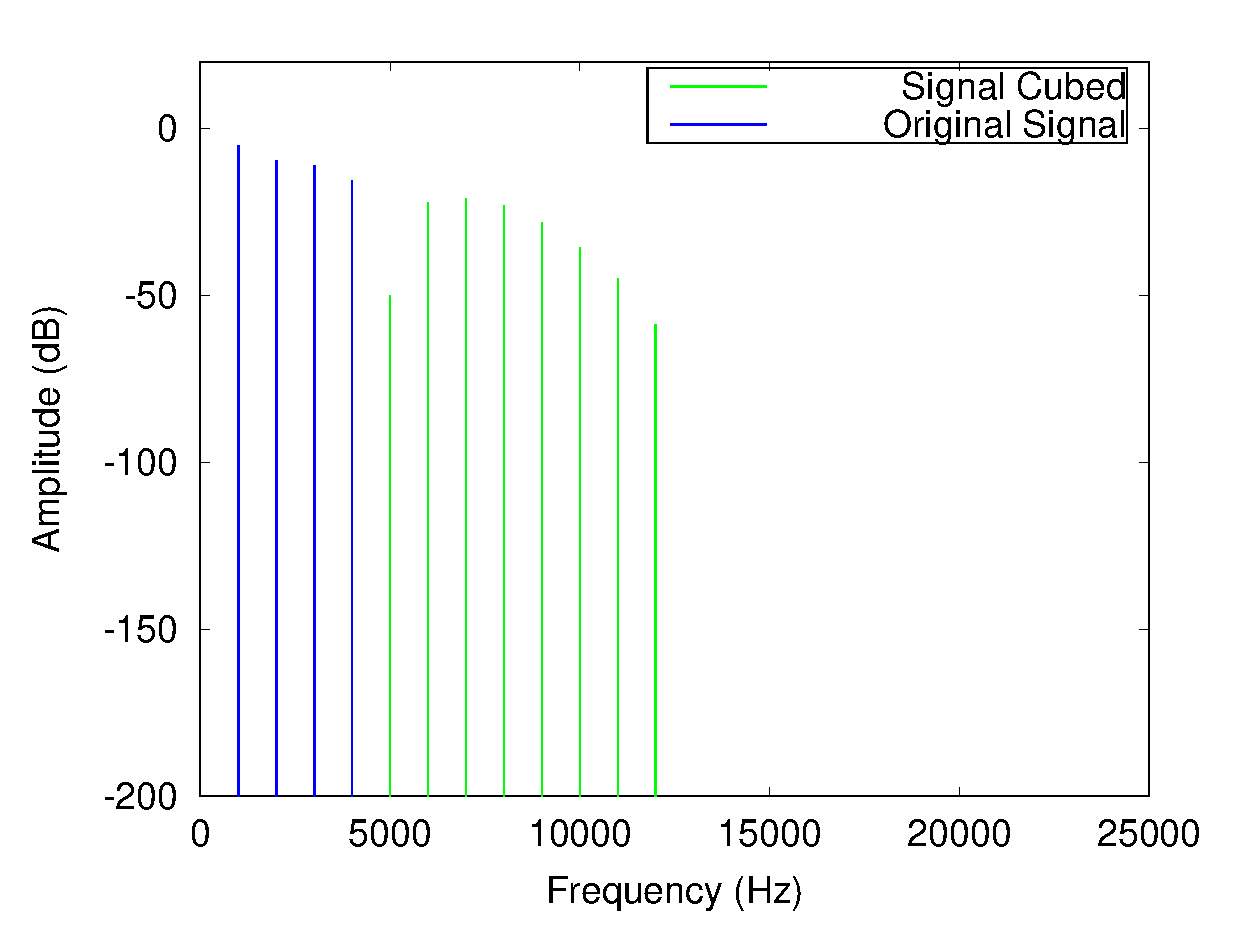
\includegraphics[width=0.6\textwidth]{chapter3/Images/CubedSpectra.eps}
				\caption{The spectral effects of cubing a signal with energy in its first four harmonics.}
				\label{fig:CubedSpectra}
			\end{figure}

			\begin{figure}[h!]
				\centering
				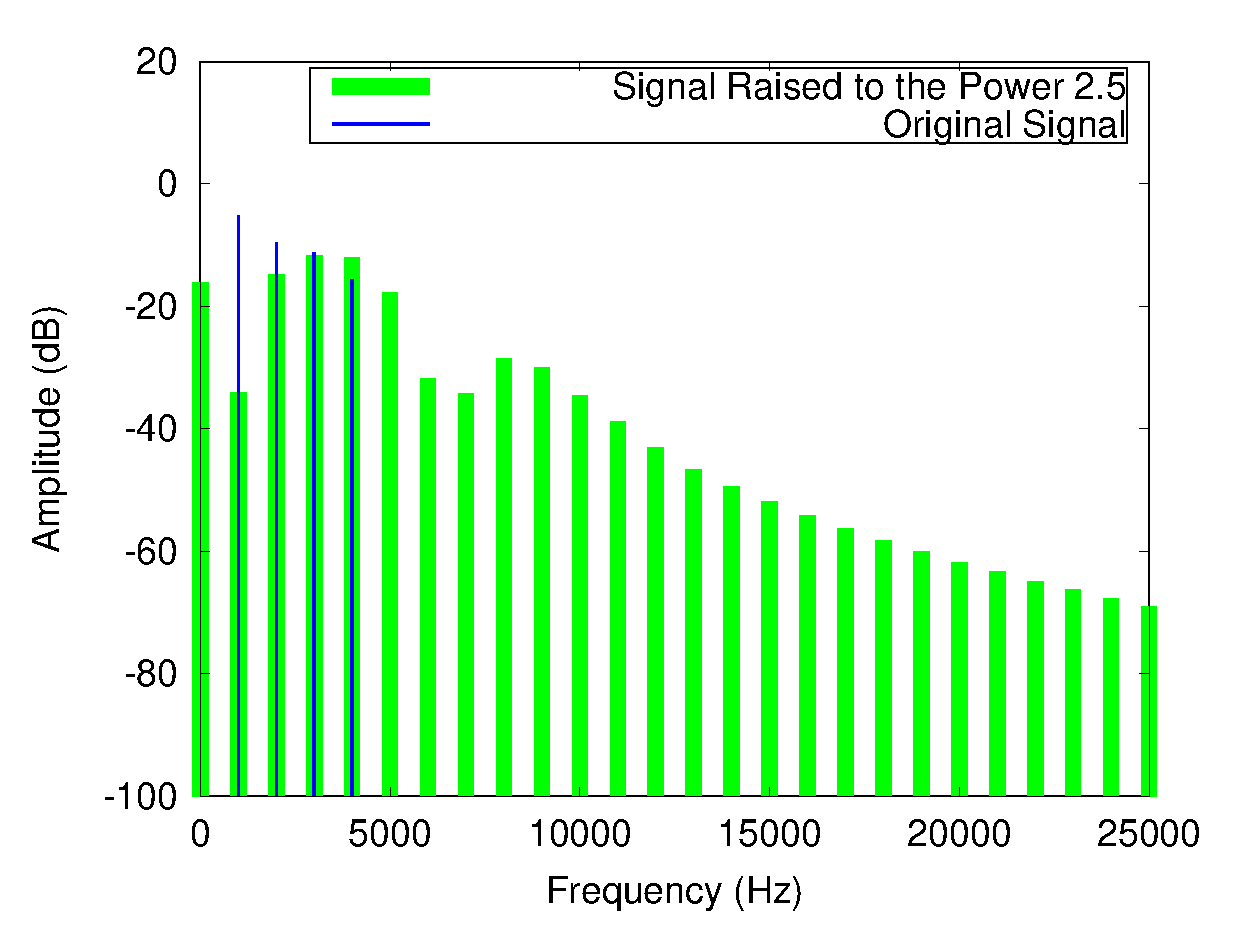
\includegraphics[width=0.6\textwidth]{chapter3/Images/RaisedToTwoAndAHalfSpectra.eps}
				\caption{The spectral effects of raising a signal with energy in its first four harmonics
					 to the power 2.5.}
				\label{fig:TwoAndAHalfSpectra}
			\end{figure}

			The highest frequency component in the original signal is 4kHz. After cubing the signal the highest
			frequency is three times this (12kHz) as seen in Figure \ref{fig:CubedSpectra}. Figure
			\ref{fig:TwoAndAHalfSpectra} shows that when the exponent is 2.5 higher frequency components are
			introduced. 

		\subsubsection*{Temporal Characteristics}
			Exponential distortion has a dynamic compression/expansion effect. For exponents greater than 1 the
			dynamics of a signal are expanded, the amplitude difference between low and high amplitude portions
			of the signal is increased. For exponents less that 1 the opposite occurs, compressing the dynamics
			of the signal. Figure \ref{fig:ExponentiationTemporalEffects} show the effects this can have on the
			attack and release portions of signals.

			\begin{figure}[h!]
				\centering
				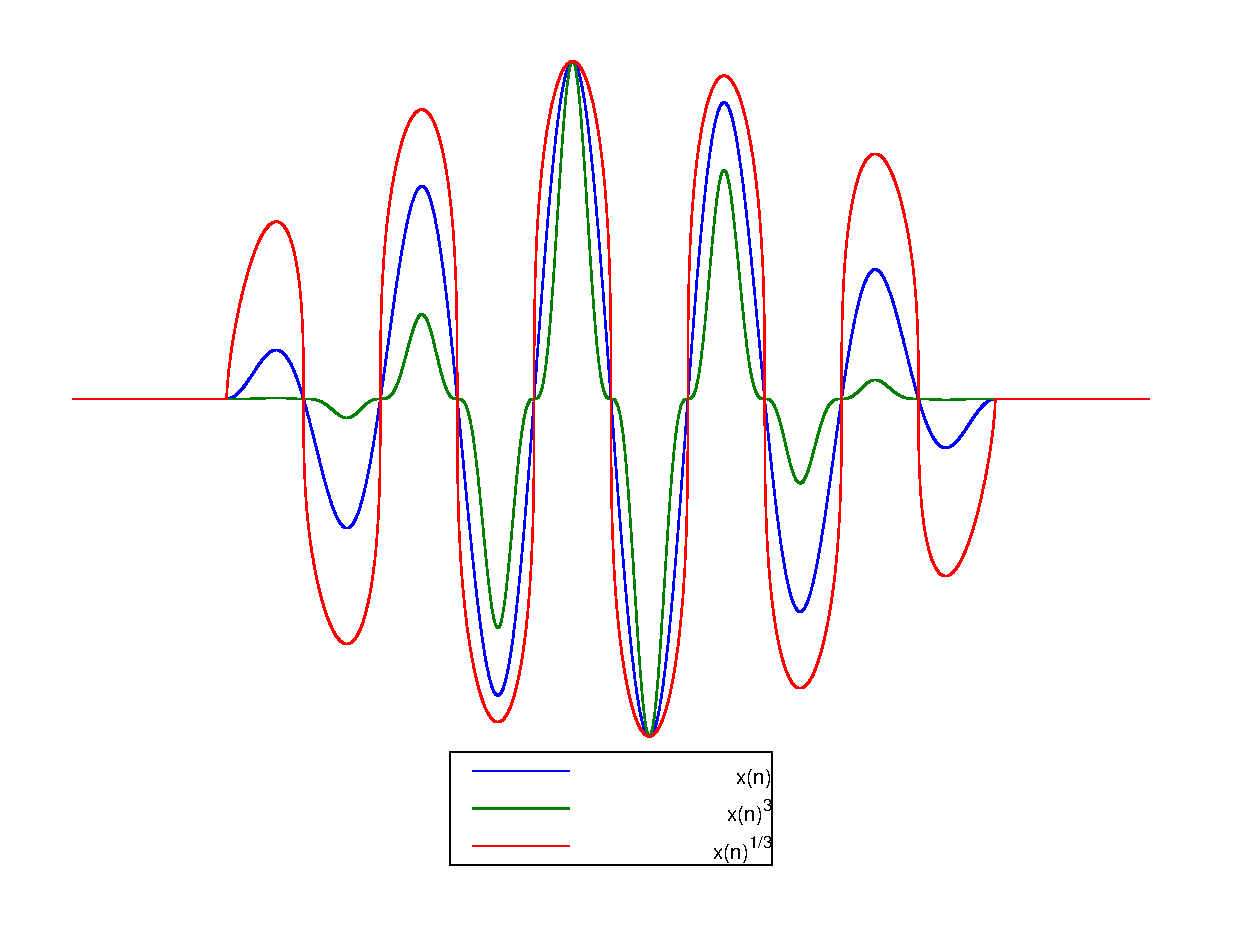
\includegraphics[width=0.6\textwidth]{chapter3/Images/ExponentiationTemporalEffects.eps}
				\caption{The temporal effects of exponential distortion.}
				\label{fig:ExponentiationTemporalEffects}
			\end{figure}

			While the time taken for the signal to rise to or decay from maximum amplitude is not changed, the
			shape of the amplitude envelope during the attack and release portions is. 

			\note
			{ 
				Probably mention the timbral effects of this in the timbre section
				\citep{patterson1994the}.
			}

		\subsubsection*{Flexibility}
			Multipliers offer greater flexibility than the previously discussed excitation methods. Control
			over the orders of distortion introduced allows for finer shaping of a signals spectrum. The output
			of several multipliers with different exponents can be summed in order to include multiple orders
			of distortion.

			Summing multiplier outputs in this way allows for approximation of other static
			nonlinearities. A low order polynomial expression approximating the desired characteristic curve
			is calculated by linear regression as shown in Figure \ref{fig:ClippingApproximation}. The
			order of the polynomial controls the maximum order of the distortion components.

			\begin{figure}[h!]
				\centering
				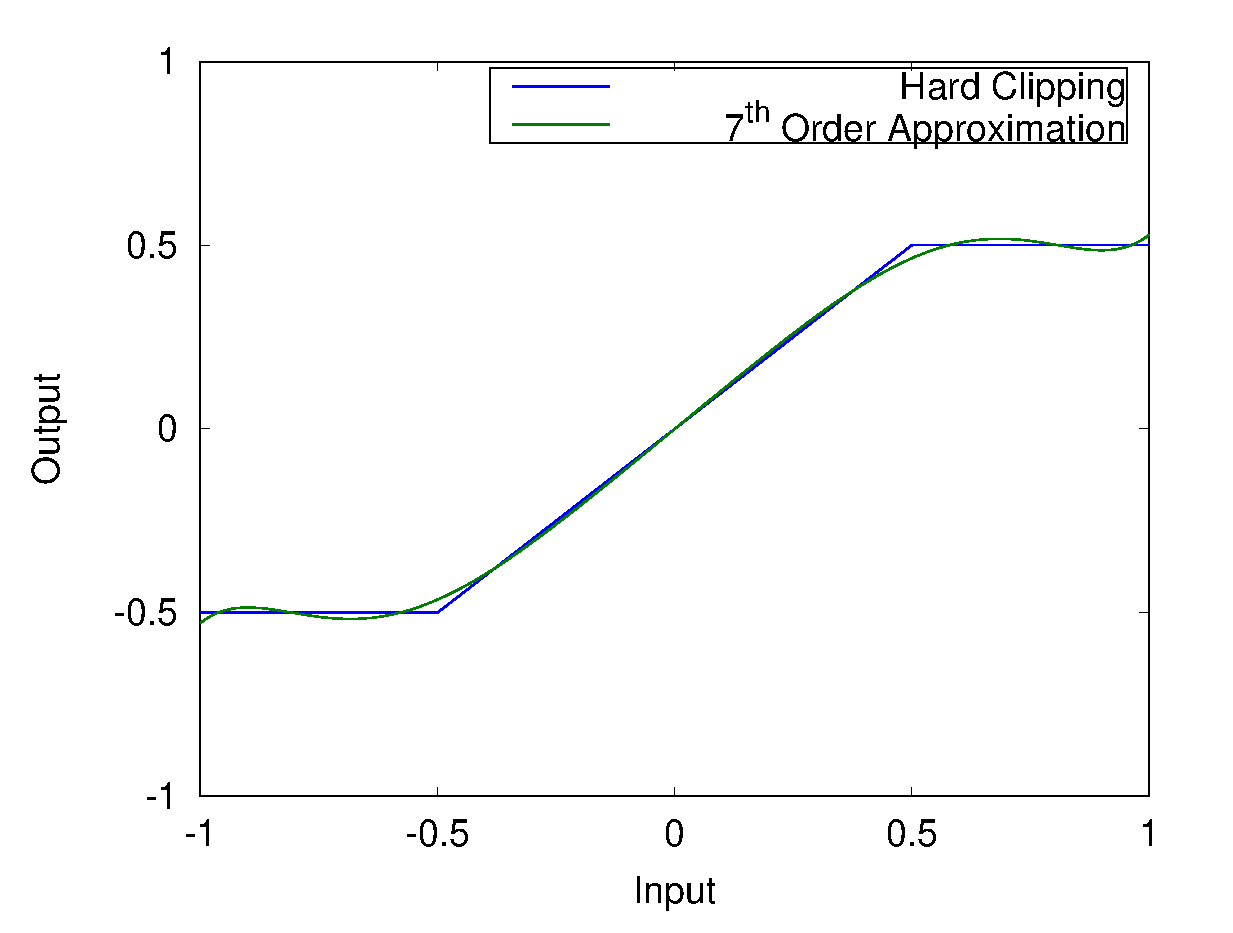
\includegraphics[width=0.6\textwidth]{chapter3/Images/ClippingApproximation.eps}
				\caption{A 7\super{th} order approximation of hard clipping using linear regression.}
				\label{fig:ClippingApproximation}
			\end{figure}

			Generating characteristic curves in this way reduces the number of aliased frequencies at the cost
			of having to evaluate a more complex polynomial to calculate the output value for each sample. A
			similar approach is undertaken by \cite{fernandez-cid2001distortion} who construct characteristic
			curves from Chebyshev polynomials in order to control the highest frequencies introduced.

%		\subsubsection*{Naturalness}

	\subsection{Single Side Band Automodulation}
	\label{sec:Excitation-SSBA}
		Single sideband automodulation (SSBA) utilises the concept of single sideband modulation
		\citep{corinthios2009signals}. This allows you to apply amplitude modulation to a signal and only produce
		either the sum or difference sideband.

		A simple way to apply single sideband modulation to a signal is through construction of an analytic signal.
		An analytic signal is a complex valued signal, the real part of which is the original signal and the
		imaginary part its Hilbert transform. The analytic signal is often denoted with a subscript letter
		$a$, such that the analytic representation of the signal $x(n)$ would be denoted $x_{a}(n)$.

		\note{This Hilbert transform stuff should probably be moved elsewhere.}

		An ideal Hilbert transform alters the phase information of a signal while leaving the magnitude information
		unchanged. Any negative frequencies in the signal have their phase shifted by $\frac{\pi}{2}$ radians.  The
		phase of positive frequencies is shifted by $-\frac{\pi}{2}$ radians. The transfer function for an FIR
		implementation of a Hilbert transform is shown in Equation \ref{eq:FirHilbertTransform}.

		\begin{equation}
			H(z) = \sum_{m = -M}^{M} \frac{2}{m\pi} sin^{2} \left( \frac{m\pi}{2} \right) z^{-m}
			\label{eq:FirHilbertTransform}
		\end{equation}

		For an ideal Hilbert transform the impulse response should be infinitely long ($M = \infty$). Practicable
		approximations of an ideal Hilbert transform can be created by using a finite value for $M$. A delay of $M$
		samples must also be introduced in order to make the filter causal. As the value of $M$ is decreased this
		delay is reduced while the magnitude response of the filter deviates further from the ideal. Figure
		\ref{fig:HilbertMagnitude} shows the magnitude responses for FIR Hilbert transform filters with $M = 11$
		and $M = 101$. The filters have a bandpass response with some ripple in the pass band. As $M$ is increased
		the bandwidth of the passband is increased and the ripple reduced. The phase response of these filters
		remains ideal no matter the value of $M$, as evidenced by Figure \ref{fig:HilbertPhase}.

		\begin{figure}[h!]
			\centering
			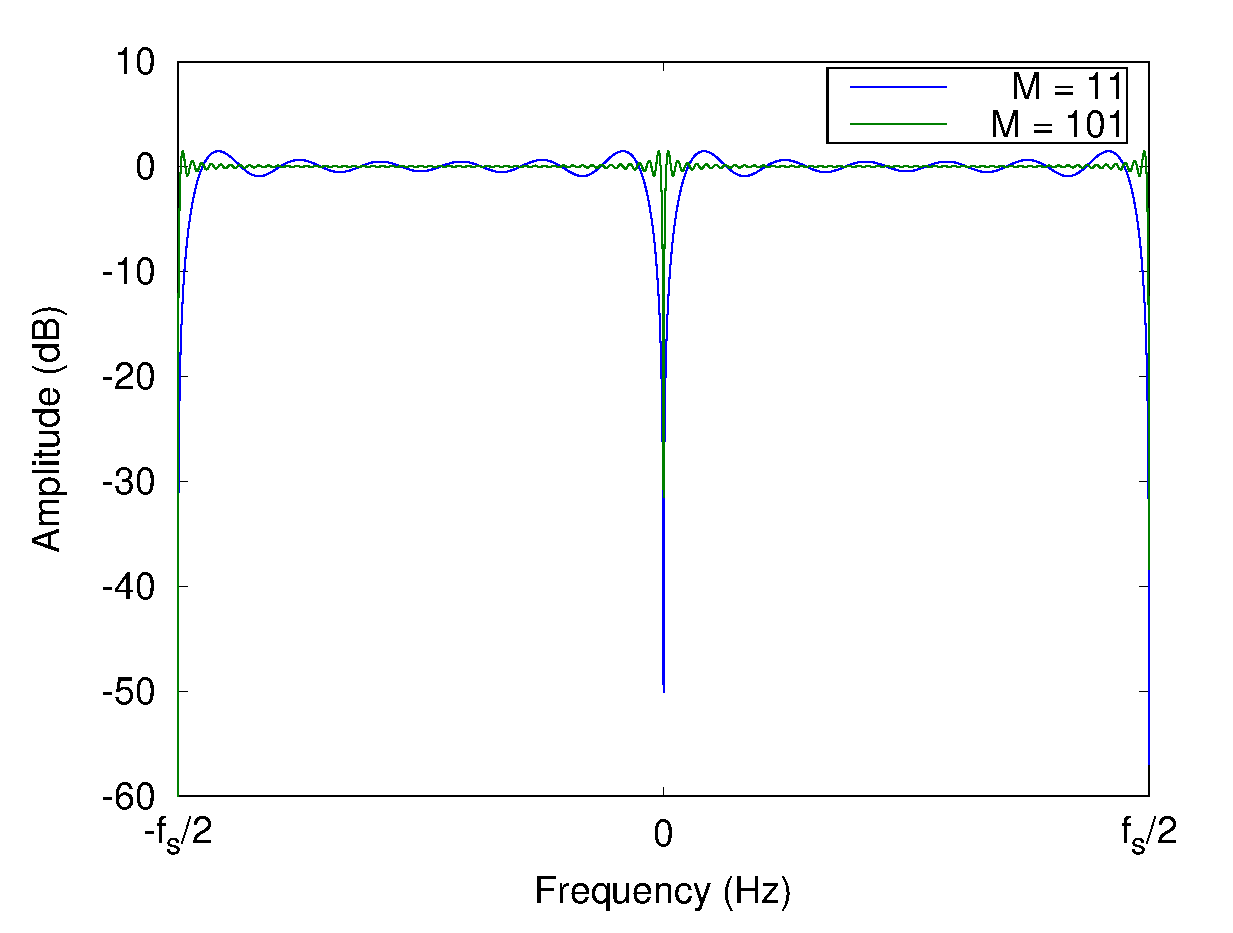
\includegraphics[width=0.6\textwidth]{chapter3/Images/HilbertMagnitudeResponses.eps}
			\caption{Magnitude responses of FIR Hilbert transform filter with different orders.}
			\label{fig:HilbertMagnitude}
		\end{figure}

		\begin{figure}[h!]
			\centering
			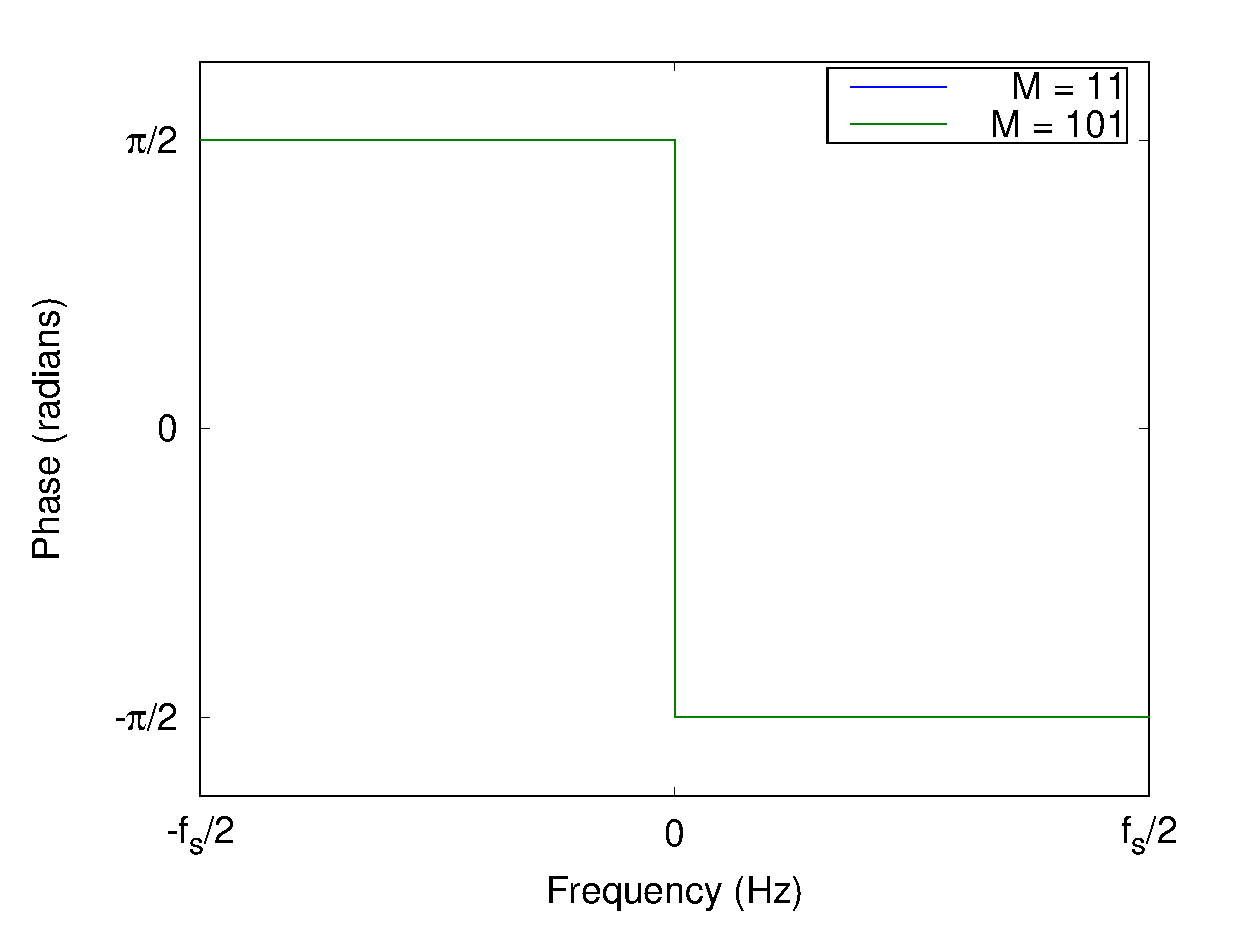
\includegraphics[width=0.6\textwidth]{chapter3/Images/HilbertPhaseResponses.eps}
			\caption{Phase responses of FIR Hilbert transform filters with different orders.}
			\label{fig:HilbertPhase}
		\end{figure}

		When using Equation \ref{eq:FirHilbertTransform} a compromise needs to be made between the tolerable amount
		of delay and the accuracy of the filter's magnitude response. Increasing $M$ will give a more accurate
		filter but introduce more delay and increase the complexity of the filter. More efficient implementations
		can be build using IIR filters if some of the properties of an ideal Hilbert transform are disregarded.

		\citet{oppenheim2014discrete} suggest constructing a phase splitter. Processing audio with two parallel
		allpass IIR filters the phase responses of which differ from each other by $\frac{\pi}{2}$ radians for a
		large proportion of the spectrum. While this is not strictly a Hilbert transform it creates two signals
		which can be used as the real and imaginary part of an analytic signal. \citet{niemitalo2003hilbert}
		provides an implementation of such a pair of filters. The phase difference between these two filters is
		seen in Figure \ref{fig:IIRHilbertPhase}.

		\begin{figure}[h!]
			\centering
			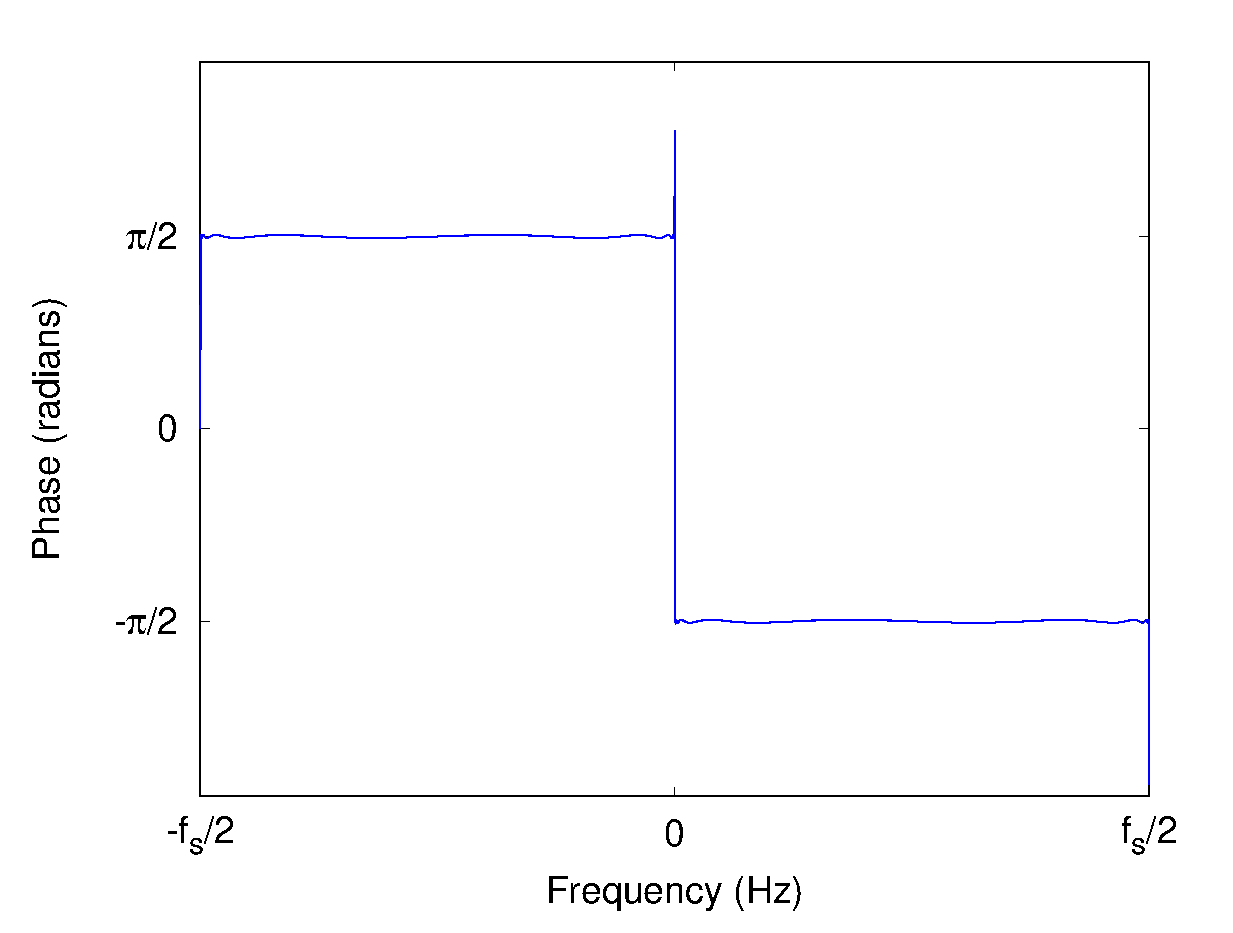
\includegraphics[width=0.6\textwidth]{chapter3/Images/IIRHilbertPhaseResponses.eps}
			\caption{The phase difference between the two allpass filters proposed by
			         \citet{niemitalo2003hilbert}.}
			\label{fig:IIRHilbertPhase}
		\end{figure}

		In single sideband automodulation the analytical representation of the input signal is multiplied with
		itself in order to generate harmonics. Equation \ref{eq:SSB} shows the $h^{\text{th}}$ order single side
		band automodulation of a signal.

		\begin{equation}
			y[n] = \Re \left( x_{a}[n]^{h} \right), \quad h \in \mathbb{N}
			\label{eq:SSB}
		\end{equation}

		\subsubsection*{Complexity}
			Compared with the harmonic excitation methods discussed previously, single side band automodulation
			has greater complexity. A Hilbert transform must be applied before a complex exponentiation
			operation for each sample. The Hilbert transform filter used must give similar response for a wide
			range of frequencies so the resulting harmonic excitation gives similar results at different
			frequencies.
			
			A high order FIR Hilbert transform filter is required to give a suitably flat magnitude response.
			A lower complexity IIR phase splitter can be used in order to reduce the computational load.
			The implementations given by \citet{niemitalo2003hilbert} consists of eight biquad filters and a
			one sample delay.
			
		\subsubsection*{Homogeneity}
			As with multipliers, SSBA is a non-homogeneous process. The amplitude envelope of the $h^{th}$
			order automodulation is the amplitude envelope of the original signal raised to the power $h$. 

		\subsubsection*{Spectral Characteristics}
			SSBA extends the control provided by multipliers as it constrains the minimum frequency introduced
			as well as the highest. Using Equation \ref{eq:SSB} only the upper side band (the sum frequencies)
			of the modulation is produced. The highest and lowest frequency components of the output are that
			of the input signal multiplied by the exponent. Between these two frequencies lie all the other
			harmonic and intermodulation components created. This can be seen in figure \ref{fig:SSBA3Spectra},
			which shows the results of applying $3^{rd}$ order SSBA to the signal used in Figures
			\ref{fig:CubedSpectra} and \ref{fig:TwoAndAHalfSpectra}. 			
			
			\begin{figure}[h!]
				\centering
				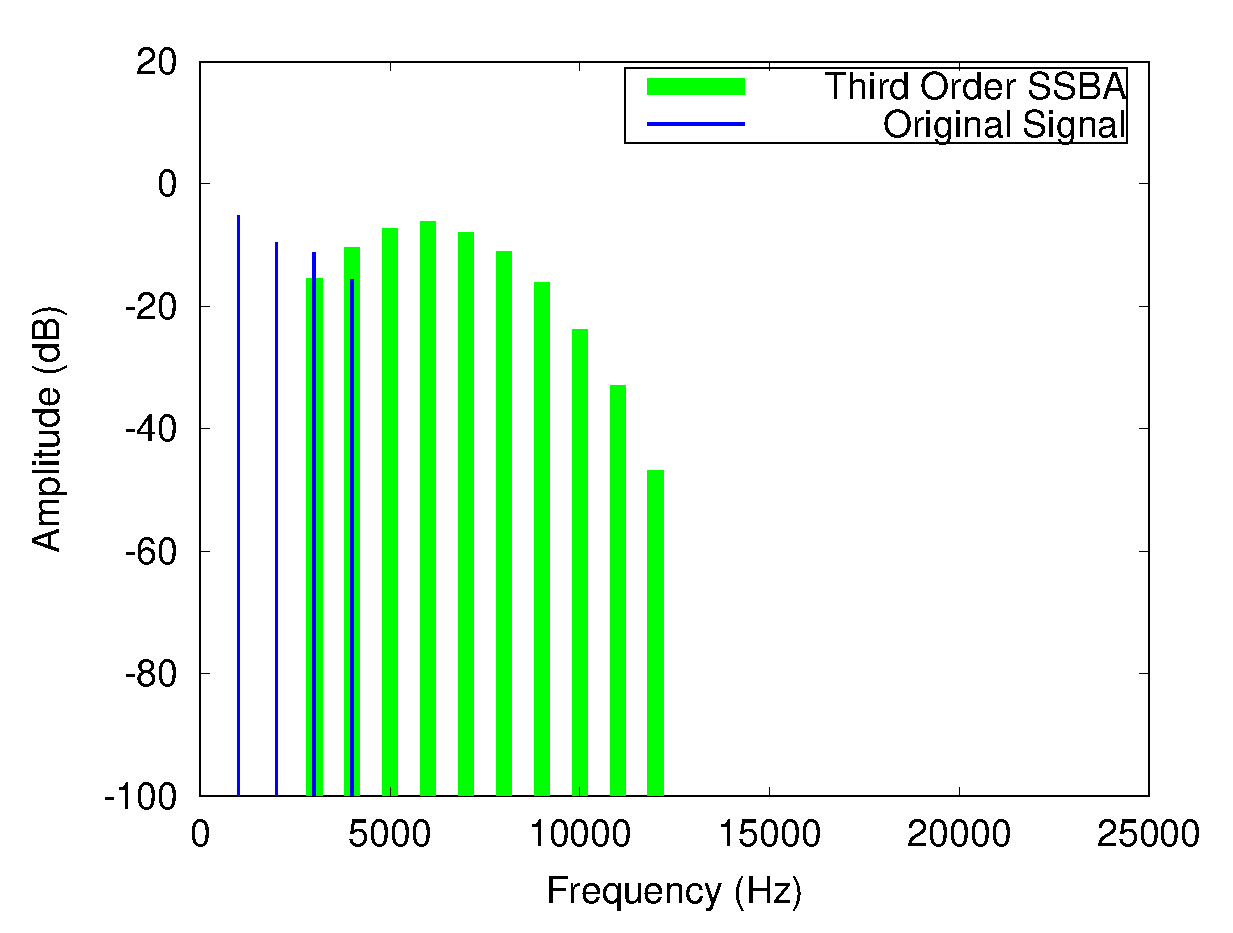
\includegraphics[width=0.6\textwidth]{chapter3/Images/SSBA3Spectra.eps}
				\caption{The spectral effects of applying third order SSBA to a signal with energy in its 
				         first four harmonics.}
				\label{fig:SSBA3Spectra}
			\end{figure}

			If aliasing does occur it is possible for the aliased frequency to lie outside of this bandwidth.
			The amplitude of aliased frequencies can be greatly reduced through filtering. Applying a low pass
			filter with a cutoff frequency of $\frac{f_{s}}{2h}$ prior to processing will reduce the amplitude
			of any frequency content in the input which will cause aliasing when processed.

		\subsubsection*{Temporal Characteristics}
			SSBA has similar temporal effects to a multiplier using an exponent greater that 1. The signal
			undergoes dynamic expansion changing the shape of its attack and release envelopes as shown in
			Figure \ref{fig:SSBATemporalEffects}.

			\begin{figure}[h!]
				\centering
				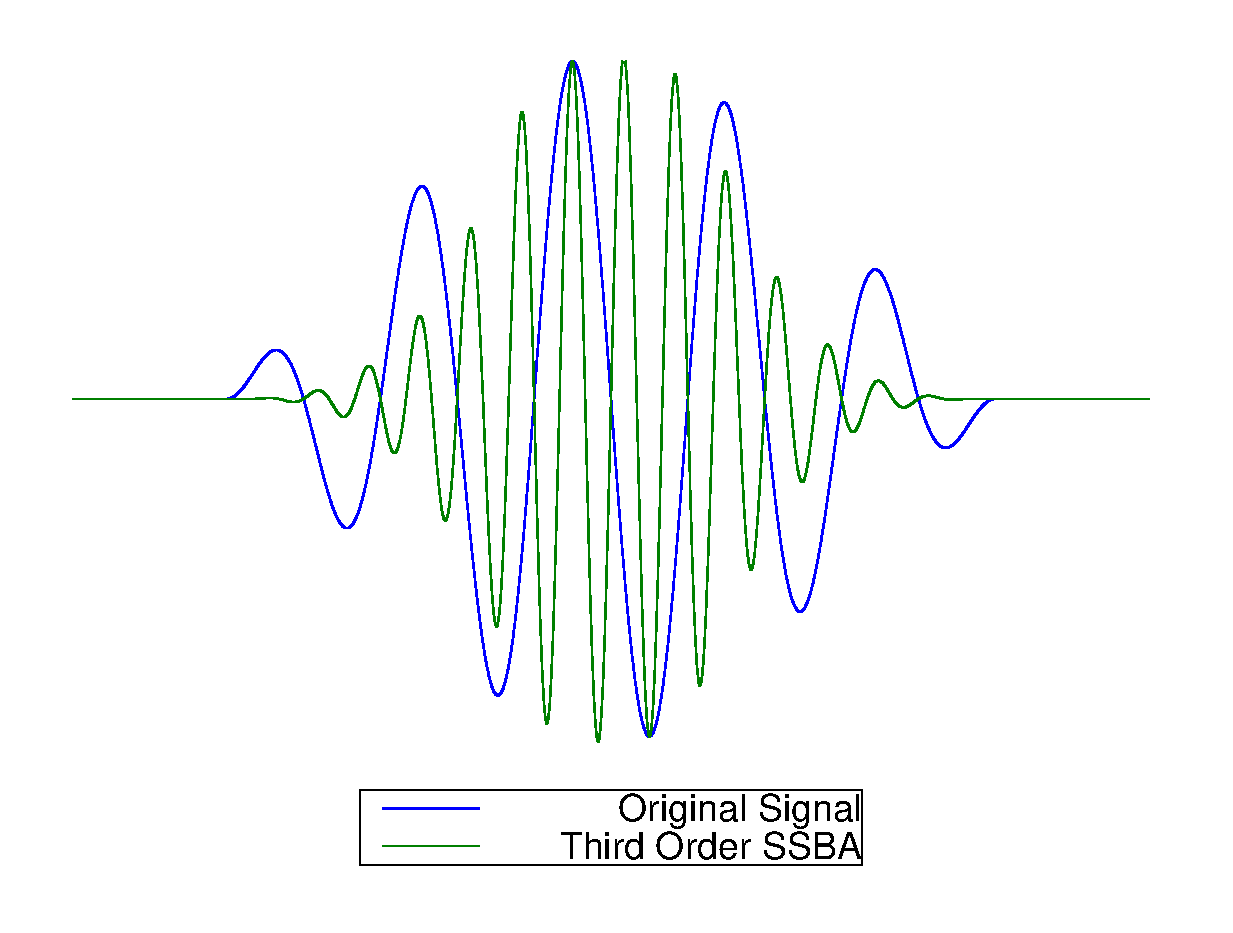
\includegraphics[width=0.6\textwidth]{chapter3/Images/SSBATemporalEffects.eps}
				\caption{The temporal effects of SSBA.}
				\label{fig:SSBATemporalEffects}
			\end{figure}

			The restricted bandwidth of the SSBA technique's output is also apparent from this graph. The input
			is a sinusoid with a simple amplitude envelope. The output is a sinusoid with 3 times the frequency
			and an amplitude envelope equal to that of the input cubed. This is in contrast to the effect of
			the multiplier shown in Figure \ref{fig:ExponentiationTemporalEffects} where the output signal is
			no longer sinusoidal.

%		\subsubsection*{Flexibility}
%		\subsubsection*{Naturalness}

	\subsection{Instantaneous Amplitude and Phase}
	\label{sec:Excitation-IAP}
		In this method, the instantaneous amplitude and phase (IAP) of the analytic signal are calculated. These
		values are then used to aid in the construction of harmonics. The instantaneous amplitude of the analytic
		signal is found by taking its absolute value, $|x_{a}[n]|$. The instantaneous phase is found by taking the
		complex argument of the analytic signal, $\arg(x_{a}[n])$. The instantaneous phase can then be scaled in
		order to scale the frequency content of the signal independent of its amplitude. Equation \ref{eq:IAP}
		shows the $h^{\text{th}}$ order instantaneous amplitude and phase modulation of a signal.

		\begin{equation}
			y[n] = |x_{a}[n]| \cos \left( h\arg(x_{a}[n]) \right), \quad h \in \mathbb{N}
			\label{eq:IAP}
		\end{equation}

		\subsubsection*{Complexity}
			The IAP technique requires a Hilbert transform to be performed before the harmonic generation. The
			computational load of this is the same as that for the SSBA technique, an IIR phase splitter
			implementation providing a good compromise between accuracy, complexity and delay. Once an analytic
			signal has been constructed the remaining processing is applied on a sample by sample basis. 
			
		\subsubsection*{Homogeneity}
			In the IAP method the magnitude and phase information of a signal are separated. The phase
			information is scaled in order to increase the frequency while the magnitude information is left
			unaltered. This preservation of magnitude information mean that the IAP method is a homogeneous
			system.
			
		\subsubsection*{Spectral Characteristics}
			In contrast to the SSBA method, the IAP method is homogeneous but provides little control over the
			bandwidth of the output when the input has multiple frequency components. Figure
			\ref{fig:IAP3Spectra} shows the spectral effects of third order IAP processing on the same signal
			used when discussing previous algorithms.

			\begin{figure}[h!]
				\centering
				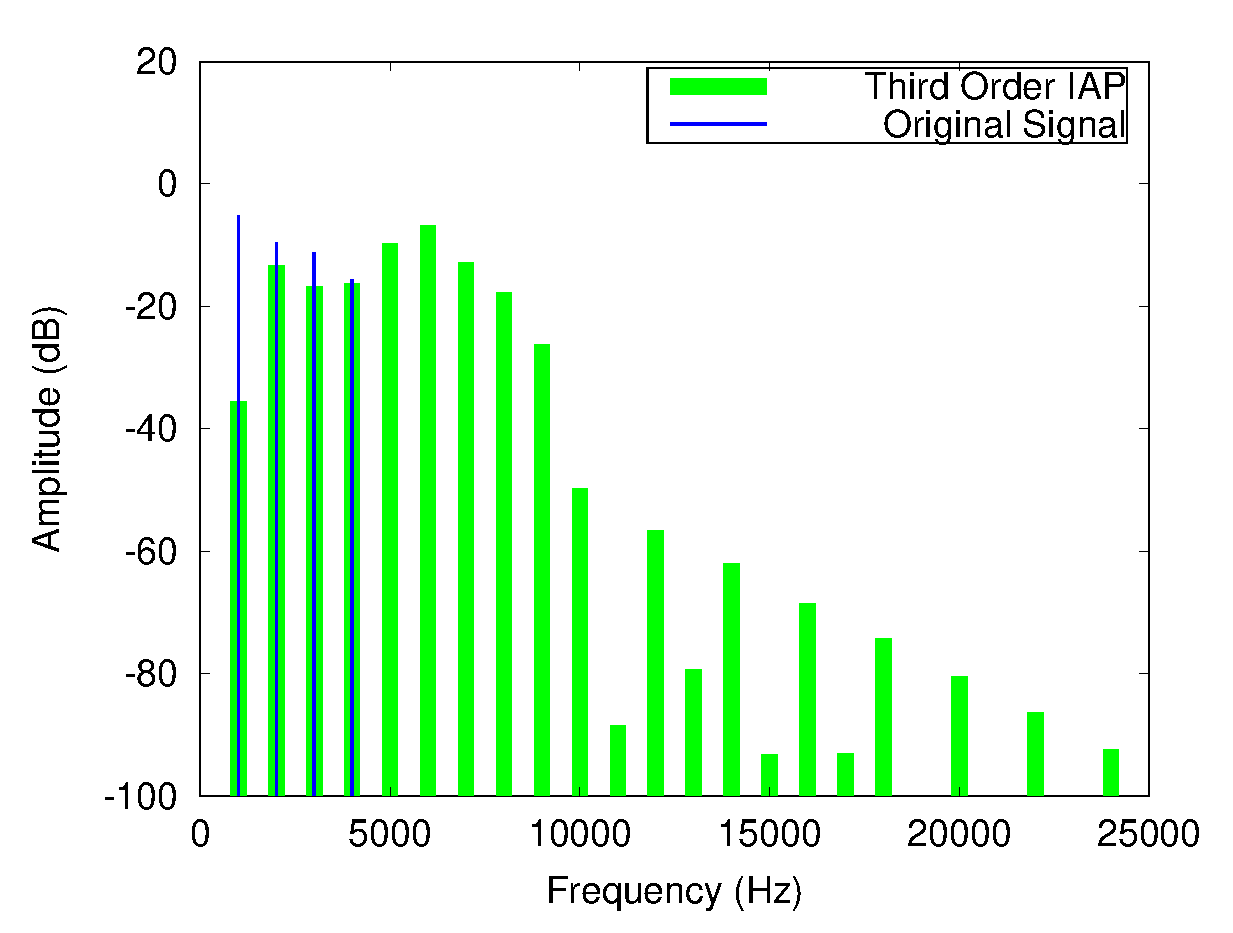
\includegraphics[width=0.6\textwidth]{chapter3/Images/IAP3Spectra.eps}
				\caption{The spectral effects of applying third order IAP to a signal with energy in its 
				         first four harmonics.}
				\label{fig:IAP3Spectra}
			\end{figure}

			When multiple frequency components are present in the input signal IAP processing produces energy
			at high order distortion components. As with previous algorithms it may be necessary to upsample
			the signal before precessing to avoid aliasing of these frequencies.

		\subsubsection*{Temporal Characteristics}
			The homogeneity of the system preserves the input signals amplitude envelope. Due to this the
			temporal characteristics of signals are unaffected. This can be seen in Figure
			\ref{fig:IAPTemporalEffects}, it is apparent that the frequency of the sinusoid has been altered
			and its amplitude envelope not.

			\begin{figure}[h!]
				\centering
				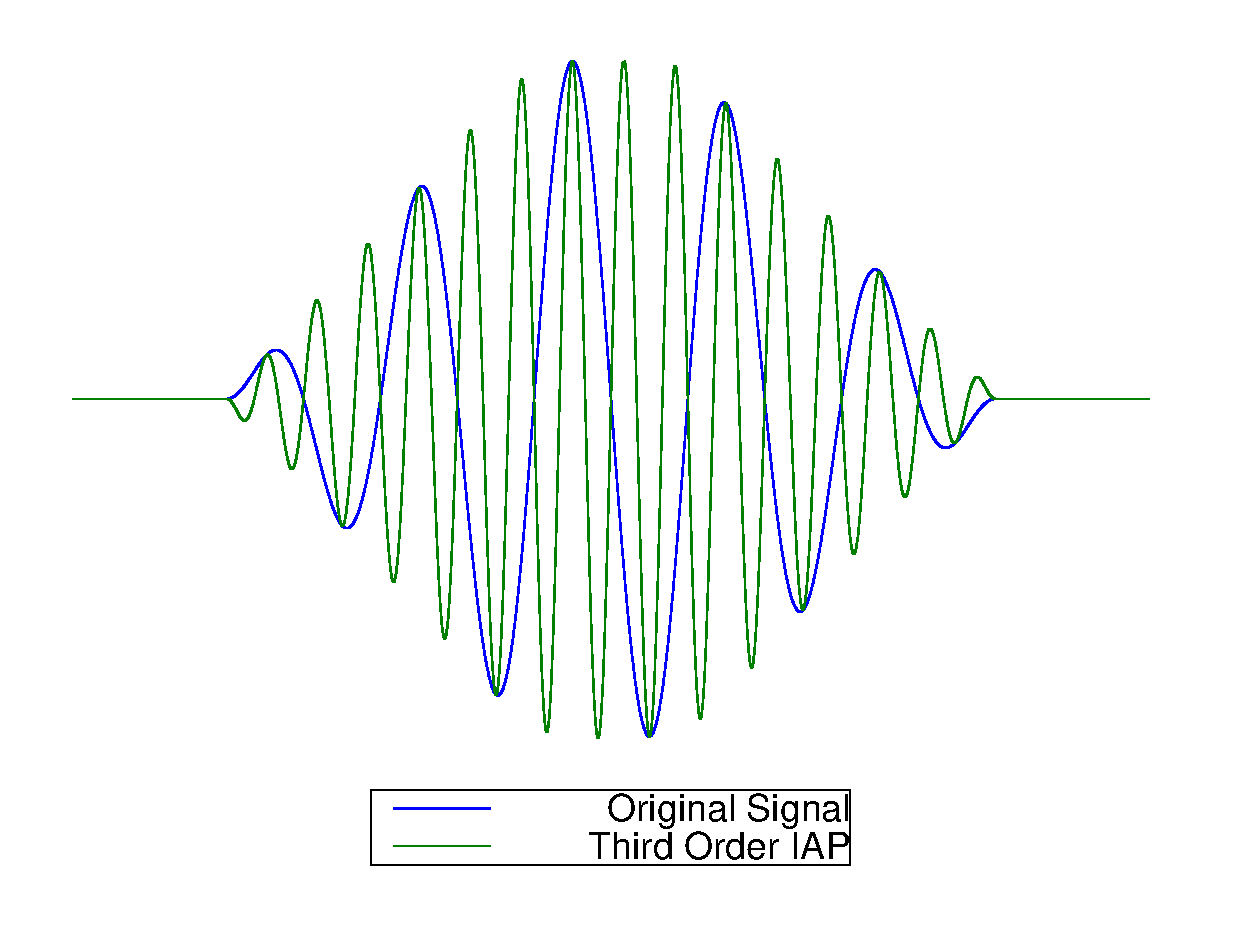
\includegraphics[width=0.6\textwidth]{chapter3/Images/IAPTemporalEffects.eps}
				\caption{The temporal effects of IAP.}
				\label{fig:IAPTemporalEffects}
			\end{figure}
			
%		\subsubsection*{Flexibility}
%		\subsubsection*{Naturalness}

	\subsection{Spectral Replication}
	\label{sec:Excitation-SpectralReplication}
		The principle behind spectral replication is to reproduce the spectral structure of a signal at higher
		frequencies as shown in Figure \ref{fig:SpectralReplication}.

		\begin{figure}[h!]
			\centering
			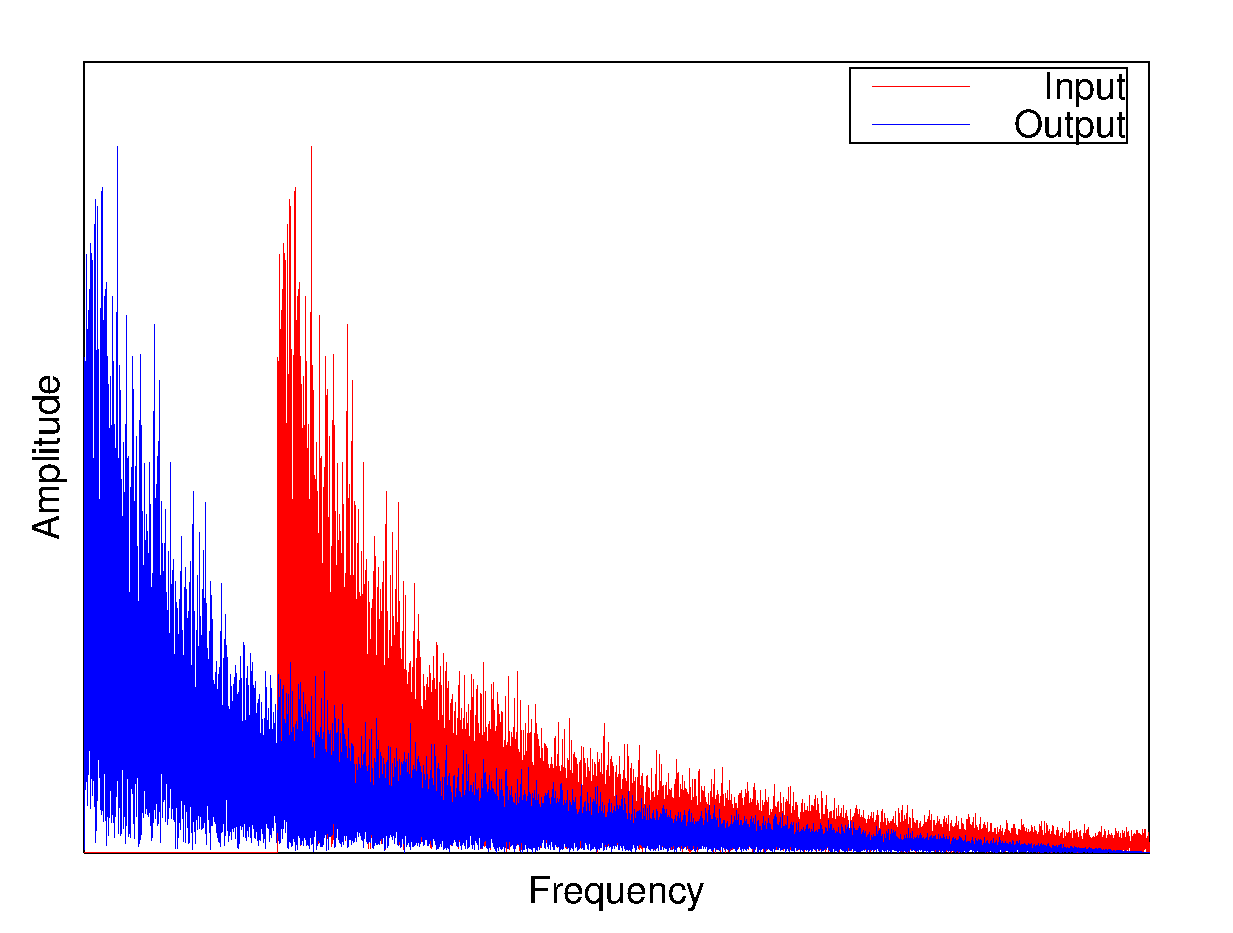
\includegraphics[width=0.6\textwidth]{chapter3/Images/SpectralReplicationSpectrum.eps}
			\caption{Reproduction of a signal at higher frequencies.}
			\label{fig:SpectralReplication}
		\end{figure}

		This spectral shift is easily implemented through the use of single side band modulation with a complex
		sinusoid as shown in Equation \ref{eq:SpectralReplication}.

		\begin{equation}
			y[n] = \Re \left( x_{a}[n] e^{2i\pi fn/ f_{s}} \right)
			\label{eq:SpectralReplication}
		\end{equation}

		Where $f$ is the amount by which the signals spectrum should be shifted.

		\subsubsection*{Complexity}
			Again, this method requires a Hilbert transform of the signal to be taken adding to the overall
			complexity of the system. After this the synthesis of a complex sinusoid needs to be carried out
			followed by the multiplication of the two complex signals on a sample by sample basis.

		\subsubsection*{Homogeneity}
			Spectral replication using Equation \ref{eq:SpectralReplication} is a homogeneous process.
			
		\subsubsection*{Spectral Characteristics}
			In spectral replication each frequency component is shifted by the same amount preserving the size
			of the spacings between them. This is useful for harmonic excitation of simple harmonically
			structured signals. Providing the spectrum is shifted by an integer multiple of the fundamental
			frequency any components at harmonic frequencies in the input will remain harmonic frequencies at
			the output. This process avoids the intermodulation distortion inherent to the systems discussed
			previously. 

			Due to every frequency component being shifted by an equal amount the bandwidth of the output is
			equal to that of the input. This predictability allows for easier control of the output spectrum.
			It also provides a simple method for reduction of aliasing. The highest frequency in the output
			will be that of the input plus the sift frequency $f$. Applying a low pass filter, with a cutoff
			frequency of $f_{s} - f$Hz to the input will help minimise the amplitude of any aliased frequency
			components.

		\subsubsection*{Temporal Characteristics}
			Spectral replication does not affect the temporal properties of a signal.

%		\subsubsection*{Flexibility}
%		\subsubsection*{Naturalness}

	\subsection{Spectral Folding}
	\label{sec:Excitation-SpectralFolding}
		Spectral folding uses upsampling in order to replicate parts of the spectrum at higher frequencies. In
		order for the output signal to have the same sampling frequency as the input the signal is 
		downsampled by a factor $k$ before being upsampled by the same factor. 
		
		To avoid aliasing during the downsampling phase the signal should have a low pass filter applied
		with a cutoff frequency of $\frac{f_{s}}{2k}$. Typically upsampling systems apply a low pass filter
		to remove any high frequency content introduced \citep{oppenheim2014discrete}. This is not needed for
		spectral folding as the production of high frequency energy is the desired result.

		After filtering, the downsampling and upsampling can be performed at the same time by retaining
		every $k^{th}$ sample and setting all others to zero. This is shown in Equation
		\ref{eq:SpectralFolding} where $x_{lf}[n]$ is the filtered input signal.		

		\begin{equation}
			y[n] = \begin{cases}
				x_{lf}[n] & \text{if $k \divides n$} \\
				0 & \text{otherwise}
			\end{cases}
			\label{eq:SpectralFolding}
		\end{equation}

		\subsubsection*{Complexity}
			Spectral folding using Equation \ref{eq:SpectralFolding} is relatively simple requiring only a low
			pass filter and some additional assignment operations. The complexity of the system as a whole
			largely depends on the complexity of the downsampling filter used.

		\subsubsection*{Homogeneity}
			Both downsampling and upsampling are homogeneous processes making spectral folding also
			homogeneous.
			
		\subsubsection*{Spectral Characteristics}
			Spectral folding with a factor $k$ results in the lowest $\frac{1}{k}$ of the input spectrum being
			repeated $k$ times in the output spectrum. Every second repetition is a mirror image of the
			original. This effect is shown in Figure \ref{fig:SpectralFolding}. 
			
			\begin{figure}[h!]
				\centering
				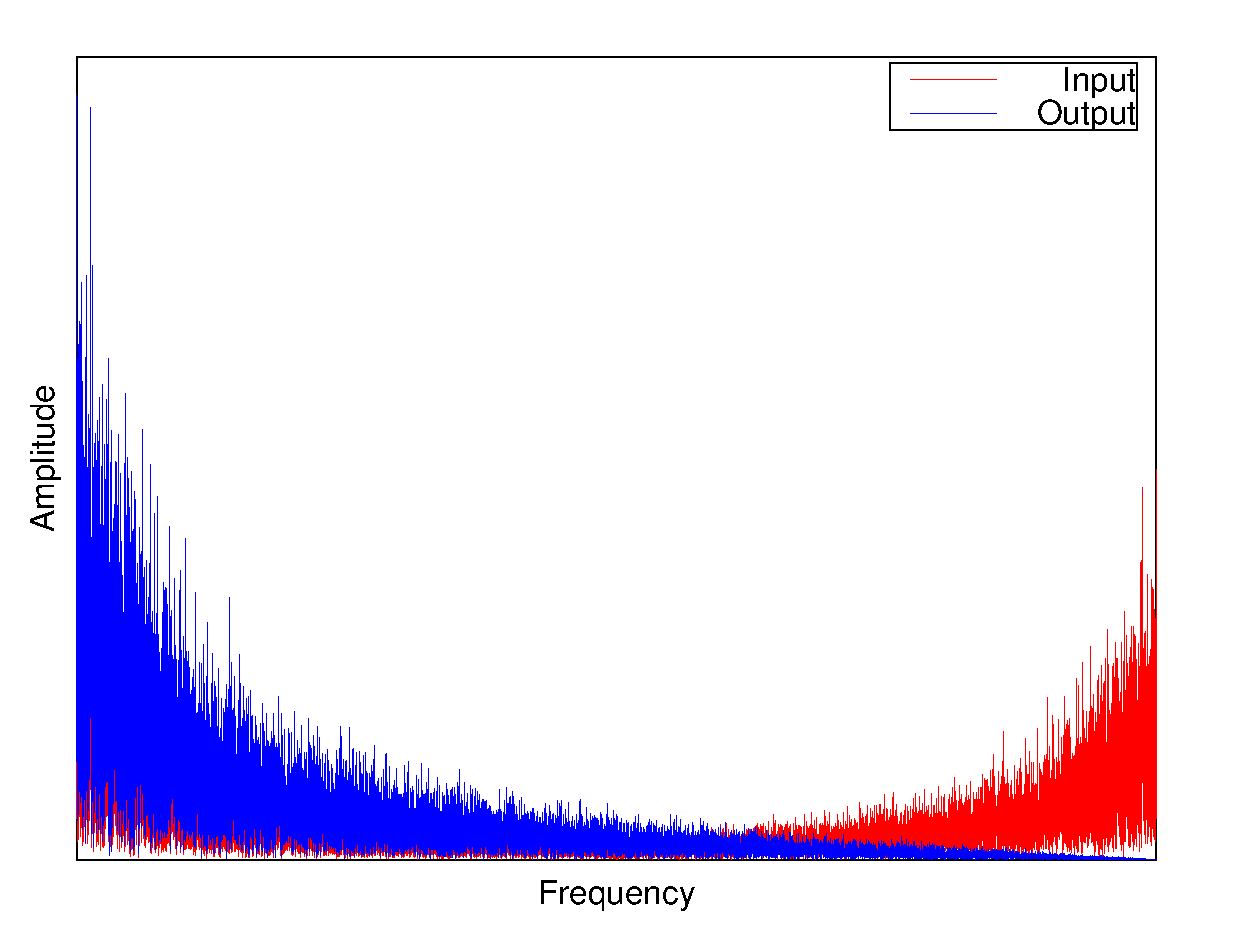
\includegraphics[width=0.6\textwidth]{chapter3/Images/SpectralFoldingSpectrum.eps}
				\caption{The spectral characteristics of spectral folding.}
				\label{fig:SpectralFolding}
			\end{figure}

			The new frequencies introduced in the output depend on the sampling rate of the signal. Unless
			$\frac{f_{s}}{2k}$ is a harmonic of the input signal there is little chance that the new
			frequencies will be harmonically related to the input.

			Other than changing the downsampling / upsampling factor, the user is given little control over the
			content of the output spectrum. The bandwidth of the output is not constricted, possibly taking up
			the entirety of the spectrum. Additional filtering is needed to shape the output spectrum as
			desired, increasing the overall complexity of the system.

		\subsubsection*{Temporal Characteristics}
			The low pass filter applied as part of the downsampling phase removes the high frequency content
			which contributes to transients in the signal. This has the effect of lengthening attack times
			similar to the effect seen in the Integrator system (Section \ref{sec:Excitation-Integrator}).

		\subsubsection*{Flexibility}
			Spectral folding is an efficient method by which to create a dense output spectrum but has many
			downsides.

%		\subsubsection*{Naturalness}

	\subsection{Spectral Stretching}
	\label{sec:Excitation-SpectralStretching}
		The principle of spectral stretching is to scale the spectrum of a signal along the frequency axis. This
		effect is shown in Figure \ref{fig:SpectralStretching}.

		\begin{figure}[h!]
			\centering
			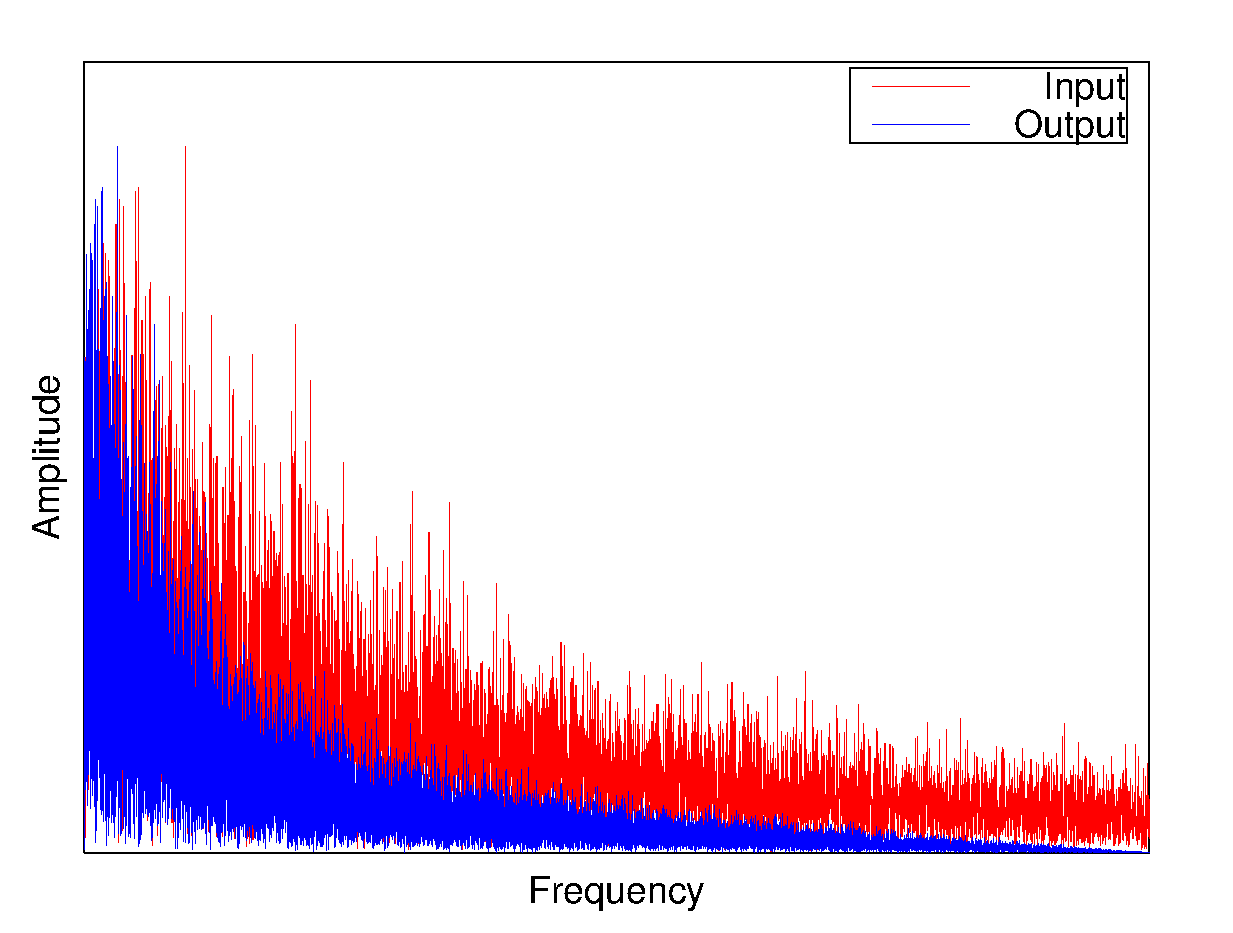
\includegraphics[width=0.6\textwidth]{chapter3/Images/SpectralStretchingSpectrum.eps}
			\caption{The spectral characteristics of spectral stretching.}
			\label{fig:SpectralStretching}
		\end{figure}

		A typical implementation of this effect utilises a phase vocoder. The phase vocoder is an algorithm which
		allows for time stretching of a signal. It is applied by calculating the short time Fourier transform of a
		signal with a given frame and hop size. The signal is then resynthesised using a different hop size in
		order to either lengthen or shorten it. This signal can then be resampled back to the length of the
		original signal scaling the frequency content in the process. 
		
		The spectrum is scaled by a factor given in Equation \ref{eq:PhaseVocoderFactor}.

		\begin{equation}
			s = \frac{h_{s}}{h_{a}}
			\label{eq:PhaseVocoderFactor}
		\end{equation}

		Where $h_{a}$ is the hop size used when calculating the STFT and $h_{s}$ is the hop size used to
		resynthesise the signal.
		
		\subsubsection*{Complexity}
			Spectral stretching using a phase vocoder require are large amount of computation. Calculating the
			STFT involves splitting the signal into frames of which the DFT is then computed. The phase
			correction for each frame must then be computed and applied before the inverse DFT of each frame is
			taken and the frames summed back together. The resulting signal then needs to be resampled
			requiring further operations. If the scaling factor is not an integer value the resampling process
			will require additional interpolation calculations.
		
			Several steps can be taken to reduce the work needed when using a phase vocoder. The computational
			complexity of the DFT calculations can be reduced by using the fast Fourier transform
			\citep{portnoff1976implementation}. When shifting the frequencies upwards the amount of work can be
			further reduced by resampling the signal before calculating the STFT \citep{laroche1999new}. This
			way there are less frames for which the DFT need be calculated.
			
		\subsubsection*{Homogeneity}
			The phase vocoder algorithm is a homogeneous system. When processing the signal in the frequency
			domain only the phase information is altered, leaving magnitude information unchanged. 

		\subsubsection*{Spectral Characteristics}
			An ideal spectral stretching system would produce the result shown in Figure
			\ref{fig:SpectralStretching}. All frequency components are scaled by the same factor. For
			harmonically structured signals this has the effect of scaling the fundamental frequency.

			The phase vocoder introduces some artefacts during its operation. The process of splitting the
			signal into frames causes spectral leakage. Energy at a given frequency is spread across the nearby
			frequencies. In a signal which only has energy at harmonic frequencies, spectral stretching by an
			integer factor will produce some inharmonic content due to this effect. Spectral leakage can be
			minimised through the use of windowing functions such as the Hamming or Blackman-Harris windows. 

			Ignoring the effect of spectral leakage, the bandwidth of the output signal will be that of the
			input multiplied by the stretching factor. This allows for effective minimisation of aliasing as
			the signal can be low pass filtered before processing as done with single side band automodulation
			(Section \ref{sec:Excitation-SSBA}).
		
		\subsubsection*{Temporal Characteristics}
			A simple phase vocoder implementation produces artefacts when processing transients in a signal.
			The phase correction stage before resynthesis can have the effect of softening the attack portion.
			The exact effect had on the transient is not able to be controlled as it depends on where the
			transient lies in the STFT frame. \citet{robel2003a} proposes a method to better process transients
			with a phase vocoder. An algorithm is used to detect the presence of transients in an STFT frame.
			The phase information is then processed differently depending on the position of the transient
			within the frame.

%		\subsubsection*{Flexibility}
%		\subsubsection*{Naturalness}

\begin{landscape}
\section{Methods Comparison}
\label{sec:Excitation-Comparison}

	\begin{tabular}{|c|c|c|c|c|c|c|}
		\hline
		\bf{Method} & \bf{Complexity} & \bf{Homogeneity} & \bf{Spectral Properties} & \bf{Temporal Properties} &
		\bf{IMD} & \bf{Flexibility} \\ % & \bf{Naturalness} \\
		\hline
		Static Nonlinearity & $\mathcal{O}(n)$ & & & & & \\
		\hline
		Rectifier & $\mathcal{O}(n)$ & & & & & \\
		\hline
		Integrator & $\mathcal{O}(n)$ & & & & & \\
		\hline
		Multiplier & $\mathcal{O}(n)$ & & & & & \\
		\hline
		SSBA & $\mathcal{O}(n)$ & & & & & \\
		\hline
		IAP & $\mathcal{O}(n)$ & & & & & \\
		\hline
		Spectral Replicator & $\mathcal{O}(n)$ & & & & & \\
		\hline
		Spectral Mirror & $\mathcal{O}(n)$ & & & & & \\
		\hline
		Spectral Stretch & $\mathcal{O}(n\log{n})$ Assuming FFT used & & & & & \\
		\hline
	\end{tabular}

\end{landscape}

\section{Harmonic Excitation Systems}
\label{sec:Excitation-Systems}
	Section \ref{sec:Excitation-Methods} covered several different methods of introducing new frequency content to a
	signal. This section will introduce techniques which can be used in conjunction with those methods to build
	harmonic excitation systems. These techniques aim to give the user more control over the new content added to the
	spectrum producing a system with can be applied to as many use cases as possible.

	\subsection{Fundamental Frequency Tracking}
	\label{sec:Excitation-Fundamental}
		The majority of the methods discussed in Section \ref{sec:Excitation-Methods} will cause intermodulation
		distortion when used on signals with multiple frequency components. As the effects of this intermodulation
		distortion can be difficult to predict it can be useful to eliminate it altogether. This should make the
		effects of a system more predictable allowing it to be used in more situations.

		An simple way to achieve this is to process only the fundamental frequency of a signal. The fundamental of
		a signal can be isolated with a filter to produce a sinusoidal signal. A harmonic excitation method is then
		used to introduce harmonics to the fundamental. As the input is sinusoidal no intermodulation components
		will be produced. This `excited' signal is then summed with the original signal to produce the output. A
		diagram of this system is shown in Figure \ref{fig:F0Tracking}.

		\begin{figure}[h!]
			\centering
			\begin{tikzpicture}
				\node (In) at (0, 1) {$x[n]$};
				\coordinate (InMid) at (1, 1);
				\draw (In) -- (InMid);

				\coordinate (Through) at (1, 0);
				\draw (InMid) -- (Through);
				\coordinate (ThroughOut) at (9.5, 0);
				\draw (Through) -- (ThroughOut);

				\coordinate (Side) at (1, 2);
				\draw (InMid) -- (Side);

				\node (F0) [draw] at (3, 2) {Fundamental Tracker};
				\node (Filter) [draw] at (3, 1) {LPF};
				\draw (InMid) -- (Filter);
				\draw (F0) -- (Filter);

				\node (Exciter) [draw] at (5.5, 1) {Harmonic Exciter};
				\draw (Filter) -- (Exciter);
				\draw (Side) -- (F0);

				\node (Add) [operator] at (9.5, 1) {+};
				\draw (ThroughOut) -- (Add);

				\node (Gain) [gain] at (8, 1) {Gain};
				\draw (Exciter) -- (Gain);
				\draw (Gain) -- (Add);

				\node (Out) at (10.5, 1) {$y[n]$};
				\draw (Add) -- (Out);

			\end{tikzpicture}
			\caption{Fundamental frequency tracking in a harmonic excitation system.}
			\label{fig:F0Tracking}
		\end{figure}


		In order to use this method the fundamental frequency of a signal must be known in order to create a filter
		to isolate it. Fundamental tracking is a widely researched field and several algorithms have been presented
		in the literature several of which are reviewed by \citet{cuadra2001efficient} and
		\citet{gerhard2003pitch}.

		Fundamental tracking can be done in both the time and frequency domains. The simplest method being to count
		the number of instances of a particular event in a given time period. This even could be a zero crossing or
		a peak or any other easily identifiable feature of the signal. As signals get more complex this method
		becomes more difficult to apply as higher frequency content will produce more instances of the event being
		counted. More advanced time domain methods include the Average Magnitude Difference Function (AMDF) and
		autocorrelation methods. Many modern fundamental tracking systems are based on these, such as the VT-AMDF
		algorithm proposed by \citet{prukkanon2009vt-amdf}.

		These methods require frame based processing which reduces the time resolution of the system. If analysing
		real time audio the current estimate of the fundamental frequency will lag behind the audio signal.
		\citet{larsen2004audio} describe a time domain frequency tracker which uses a simple recursive formula.
		While this is not a accurate as the more advanced techniques it takes considerably less time to compute.

		Frequency domain methods require the DFT of the signal to be calculated introducing considerable
		complexity. Widely used frequency domain techniques include the Harmonic Product Spectrum (HPS) and maximum
		likelihood methods.

		For real time harmonic excitation the accuracy of the fundamental tracking algorithm is not as important as
		it is in other fields such as automatic music transcription. The aim of the system in Figure
		\ref{fig:F0Tracking} is to reduce the level of higher harmonics compared to the fundamental. Using a low
		pass filter with a cutoff frequency close to the fundamental will achieve this. The lag between the audio
		and the estimate of the fundamental frequency is of more concern. The system needs to respond quickly to
		changes in fundamental frequency in order to better isolate the fundamental for processing.

		A problem is posed by signals with little energy at their fundamental frequency such as those produce in
		the lower register of a Double Bass \citep{askenfelt2010double}. A fundamental tracking algorithm will
		still return the frequency of the fundamental despite its low magnitude. The output of the filter may then
		have to little amplitude to be of any use for harmonic excitation. A frequency domain approach to
		fundamental tracking may be more robust in this situation as it can easily be check whether there is
		sufficient energy at the detected fundamental frequency. If there is not, the first harmonic which has
		sufficient magnitude can be isolated and used as the input to the exciter. If this action is taken only the
		spectral replication and spectral shifting methids will allow for the excitation of evey harmonic as the
		SSBA and IAP methods only allow for integer multiplications of the frequency.

		The system shown in Figure \ref{fig:F0Tracking} can provide differing levels of flexibility depending on
		the harmonic exciter used. Using a simple clipper it will generate a series of harmonics of the
		fundamental. Using methods which provide more control over the order of distortion allows users to excite
		single harmonics in the output. This will be covered in the next section.

	\subsection{Individual Harmonic Generation}
	\label{sec:Excitation-Individuals}
		Control over which harmonics are excited in a signal can be achieved by exciting individual harmonics. The
		principle behind this is to isolate the fundamental and then shift its frequency to that of the desired
		harmonic. This can be achieved using the SSBA, IAP, Spectral Replication and Spectral Stretching methods.
		The output spectrum can be shaped as desired by generating several different harmonics in this manner and
		summing them together.
		
		\citet{bregman1994auditory} suggests that when presented with an auditory scene the human hearing system
		separates out sources by grouping like harmonics together. Whether harmonics are deemed to be similar
		depends on their frequency and amplitude envelope. When applying harmonic excitation it is necessary to
		ensure that the newly introduces harmonic content will be judged as similar to the existing content. If not
		the excited harmonics may be perceived as a new sound source rather than contributing towards changing the
		timbre of a sound. Any system which generates new harmonic content and then sums it back into the original
		signal is at risk of this occurring. When generating multiple harmonics individually and summing them all
		together this risk is increased.

		An experiment was conducted to evaluate which harmonic excitation method is best suited to the generation
		of individual harmonics. A primary aim of this experiment was to determine whether any of the methods would
		cause a tone from a single instrument to be perceived as coming from multiple sources. Each method was used
		to reconstruct signals which from which some harmonic content had been removed. The quality of the
		reconstruction was assessed by participants in a multiple stimulus listening test. 

		The audio samples each consisted of a single instrument playing a sustained tone. The instruments used
		were:
		
		\begin{itemize}
			\item A bowed cello.
			\item A clarinet.
			\item A synthesised harmonic sound.
			\item A piano.
		\end{itemize}

		For each sample the third through ninth harmonics were removed. Spectrograms of the cello sample before and
		after this process are shown in Figures \ref{fig:CelloSpectrogram} and \ref{fig:CelloFilteredSpectrogram}.
		Test stimuli were then created by reintroducing these harmonics using SSBA, IAP and a synthesis method.
		The synthesis method consisted of using the STFT to measure the amplitude envelope of the fundamental
		frequency and applying this to a synthesised sine wave at the frequency of the desired harmonic. 

		\begin{figure}[h!]
			\centering
			\subfloat[Unprocessed Sample]
			{
				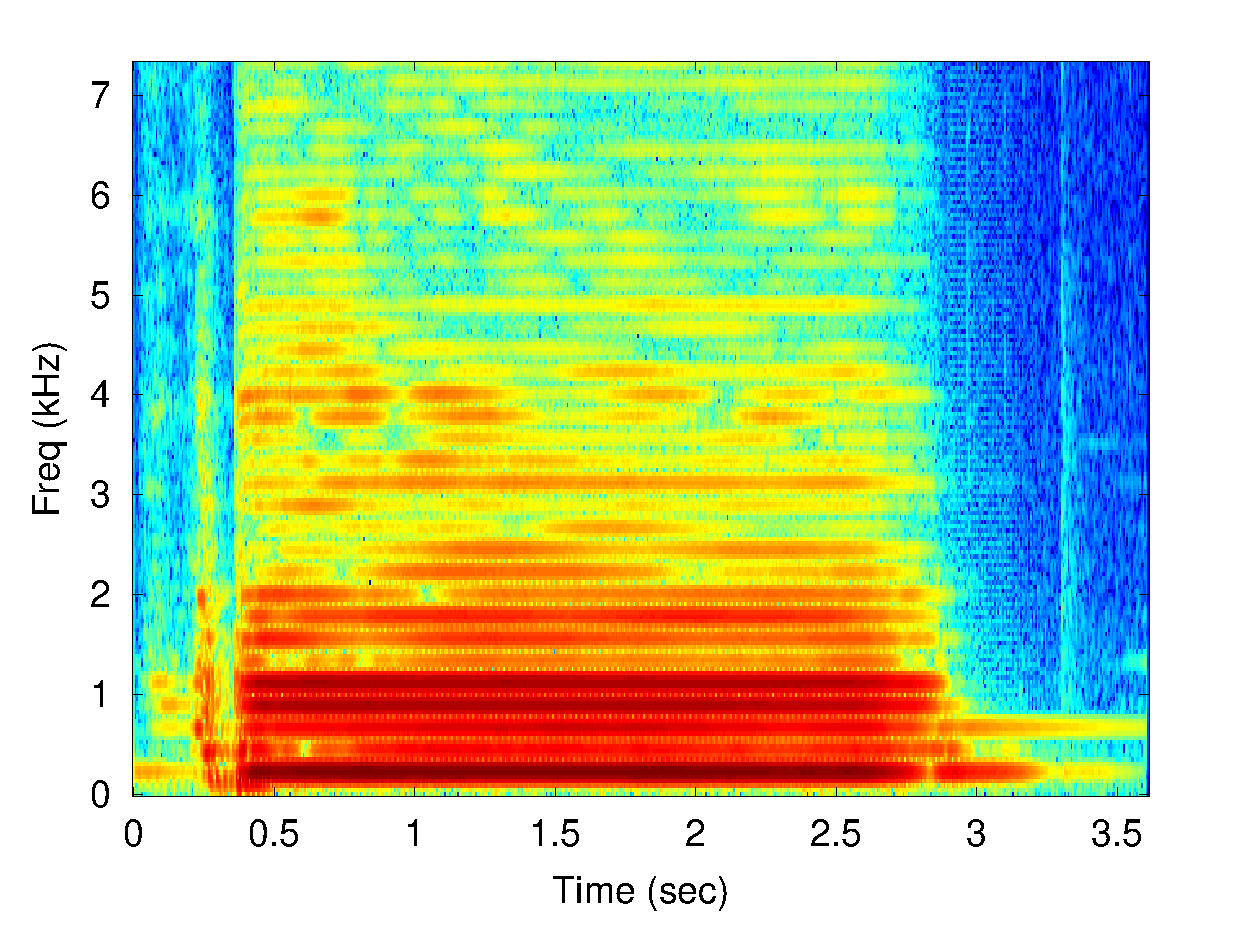
\includegraphics[width=0.45\textwidth]{chapter3/Images/CelloSpectrogram.eps}
				\label{fig:CelloSpectrogram}
			}
			\qquad
			\subfloat[Filtered Sample]
			{
				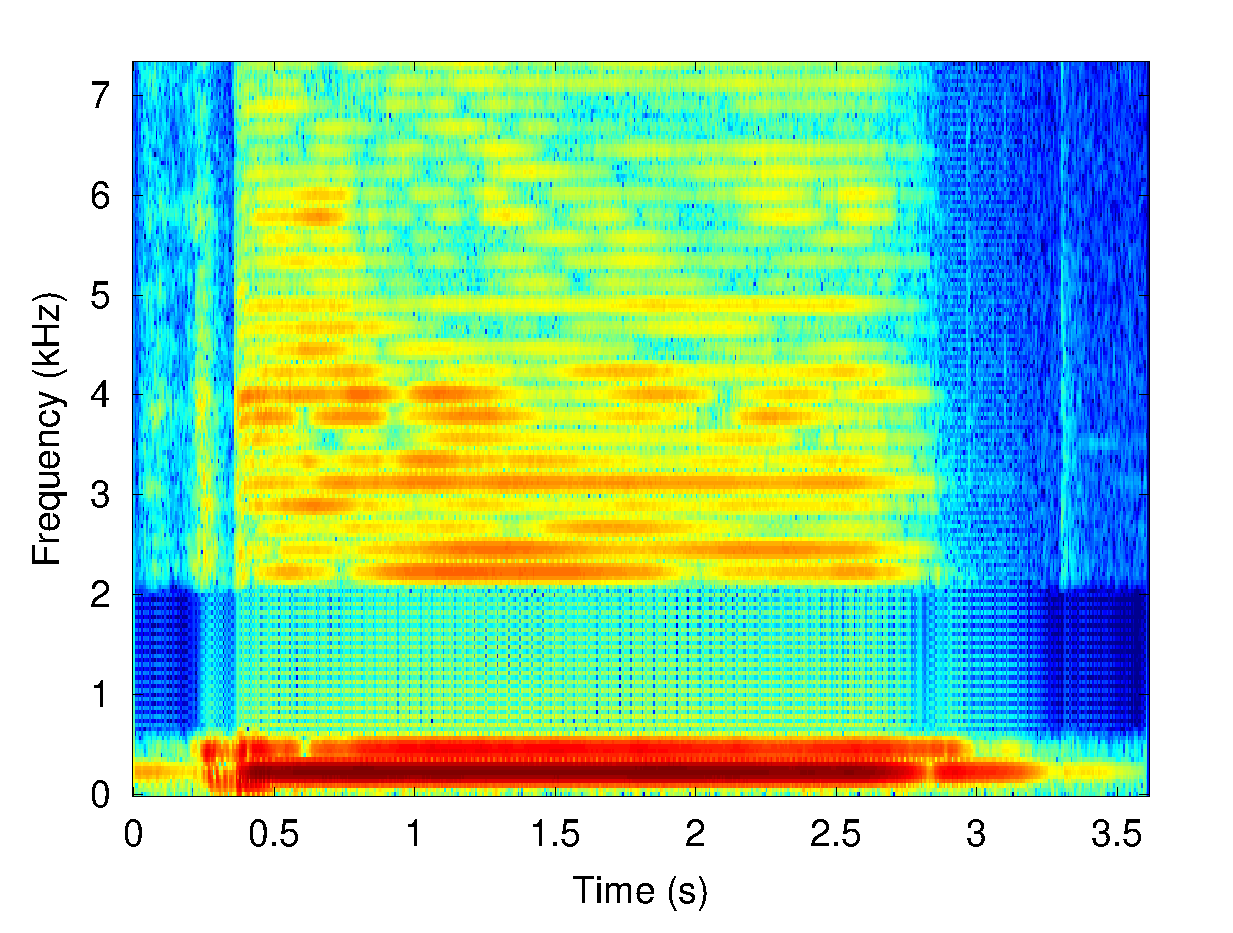
\includegraphics[width=0.45\textwidth]{chapter3/Images/CelloFilteredSpectrogram.eps}
				\label{fig:CelloFilteredSpectrogram}
			}
			\caption{Spectrograms of the cello sample.}
			\label{fig:CelloSpectrograms}
		\end{figure}

		Each sample was reconstructed three times using each method, using different parameters each time. For the
		SSBA and IAP methods a different order FIR filter was used to isolate the fundamental frequency. The
		filters used had orders of 50, 100 and 500. For the synthesis method the window length of the STFT was
		changed, taking values of 50, 100 and 500 samples. Spectrograms for the reconstructed samples using the
		smallest filter order / STFT window length are shown in Figure \ref{fig:ReconstructedCelloSpectrograms}.

		\begin{figure}[h!]
			\centering
			\subfloat[SSBA with a 50\super{th} order filter.]
			{
				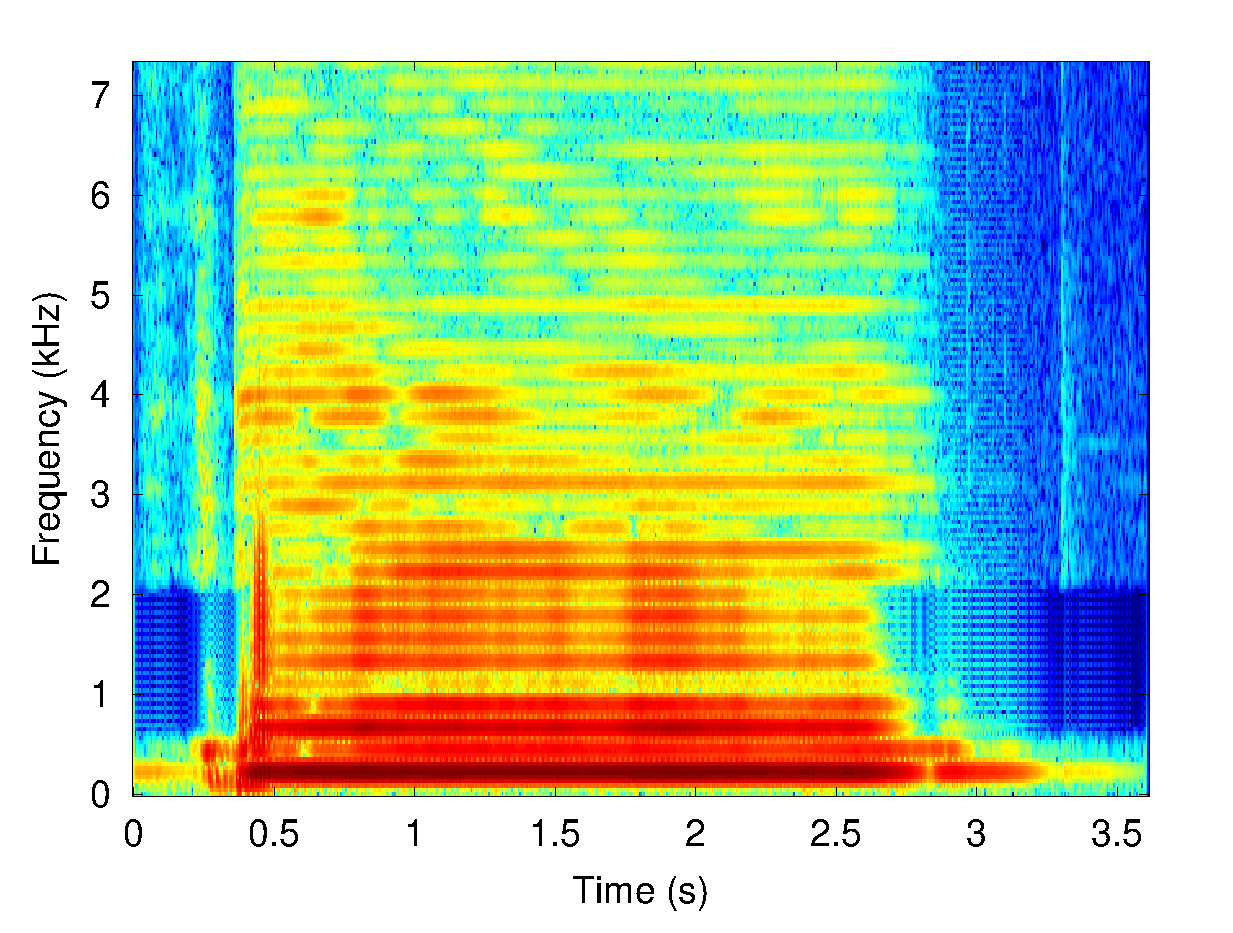
\includegraphics[width=0.45\textwidth]{chapter3/Images/CelloSSBASpectrogram.eps}
				\label{fig:CelloSSBASpectrogram}
			}
			\qquad
			\subfloat[IAP with a 50\super{th} order filter.]
			{
				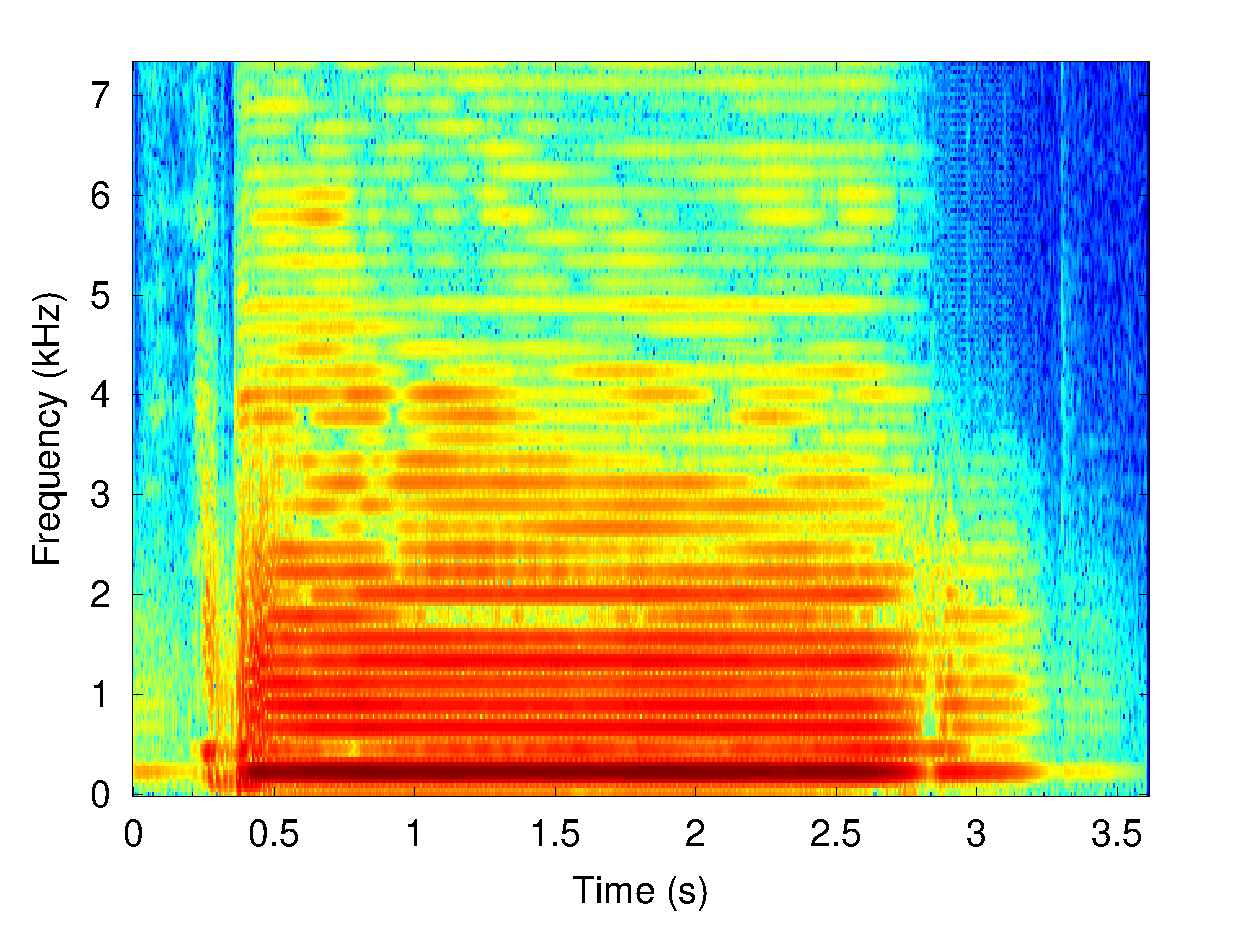
\includegraphics[width=0.45\textwidth]{chapter3/Images/CelloIAPSpectrogram.eps}
				\label{fig:CelloIAPSpectrogram}
			}
			
			\subfloat[Synthesis with an STFT window length of 50 samples.]
			{
				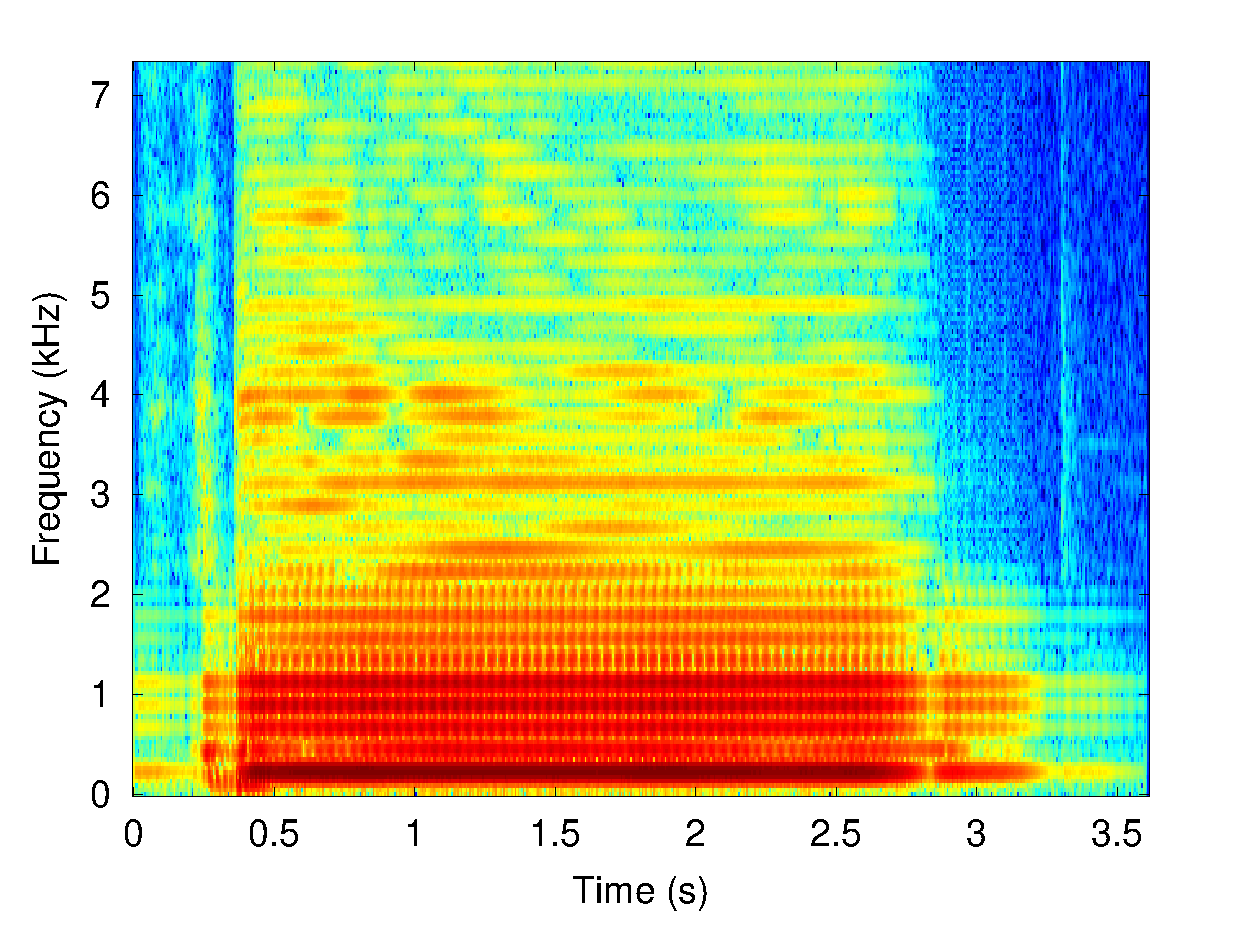
\includegraphics[width=0.45\textwidth]{chapter3/Images/CelloSynthesisSpectrogram.eps}
				\label{fig:CelloSynthesisSpectrogram}
			}
			\caption{Spectrograms of the cello sample reconstructed using three different methods.}
			\label{fig:ReconstructedCelloSpectrograms}
		\end{figure}

		On inspection of these spectrograms the characteristics of the three excitation methods can be seen. The
		amplitude envelopes of the generated harmonics differ greatly between the methods. Comparing the decay
		portion of the envelopes compared with those in the original signal (Figure \ref{fig:CelloSpectrogram})
		highlights these differences. In the cello sample the fundamental frequency and third harmonic have a
		longer decay time then the other harmonics. The harmonics generated by the IAP and synthesis methods
		(Figures \ref{fig:CelloIAPSpectrogram} and \ref{fig:CelloSynthesisSpectrogram}) use the amplitude envelope
		of the fundamental frequency extending the decay time of the these harmonics compared to that in the
		original. Those generated by the SSBA method (Figure \ref{fig:CelloSSBASpectrogram}) have shortened decay
		times. As the order of the harmonic is increased the decay time gets shorter due to the dynamic expansion
		shown in Figure \ref{fig:SSBATemporalEffects}.

		The amplitude envelopes of the harmonics generated using the synthesis techniques exhibit a large amount of
		ripple. This is due to the amplitude of the fundamental being calculated in blocks. These inaccuracies are
		not present in the harmonics generated using the IAP method as the amplitude is calculated on a sample by
		sample basis.

		Test participants were presented with all processed version of a particular sample at once along with a
		reference stimulus (the unprocessed sample) and an anchor stimulus (the sample with its harmonics removed).
		Participants were asked to grade how well each processed stimulus recreated the reference stimulus on a
		scale from 0 to 100.

		The results of this experiment are shown in Figure \ref{fig:SMCResults} with error bars showing the 95\%
		confidence intervals. The stimuli numbers refer to different processing algorithms as follows.

		\begin{tabular}{>{\bfseries}cl}
			1. & Reference Stimulus \\
			2. & Sample reconstructed using the synthesis method with an STFT window length of 50
			     samples. \\
			3. & Sample reconstructed using the synthesis method with an STFT window length of 100
			     samples. \\
			4. & Sample reconstructed using the synthesis method with an STFT window length of 500
			     samples. \\
			5. & Sample Reconstructed using the SSBA method using a 50\super{th} order filter.\\
			6. & Sample Reconstructed using the SSBA method using a 100\super{th} order filter.\\
			7. & Sample Reconstructed using the SSBA method using a 500\super{th} order filter.\\
			8. & Sample Reconstructed using the IAP method using a 50\super{th} order filter.\\
			9. & Sample Reconstructed using the IAP method using a 100\super{th} order filter.\\
		     	10. & Sample Reconstructed using the IAP method using a 500\super{th} order filter.\\
	     		11. & Sample with third through ninth harmonics removed (anchor).\\
		\end{tabular}

		\begin{figure}[h!]
			\centering
			\subfloat[Cello Sample]
			{
				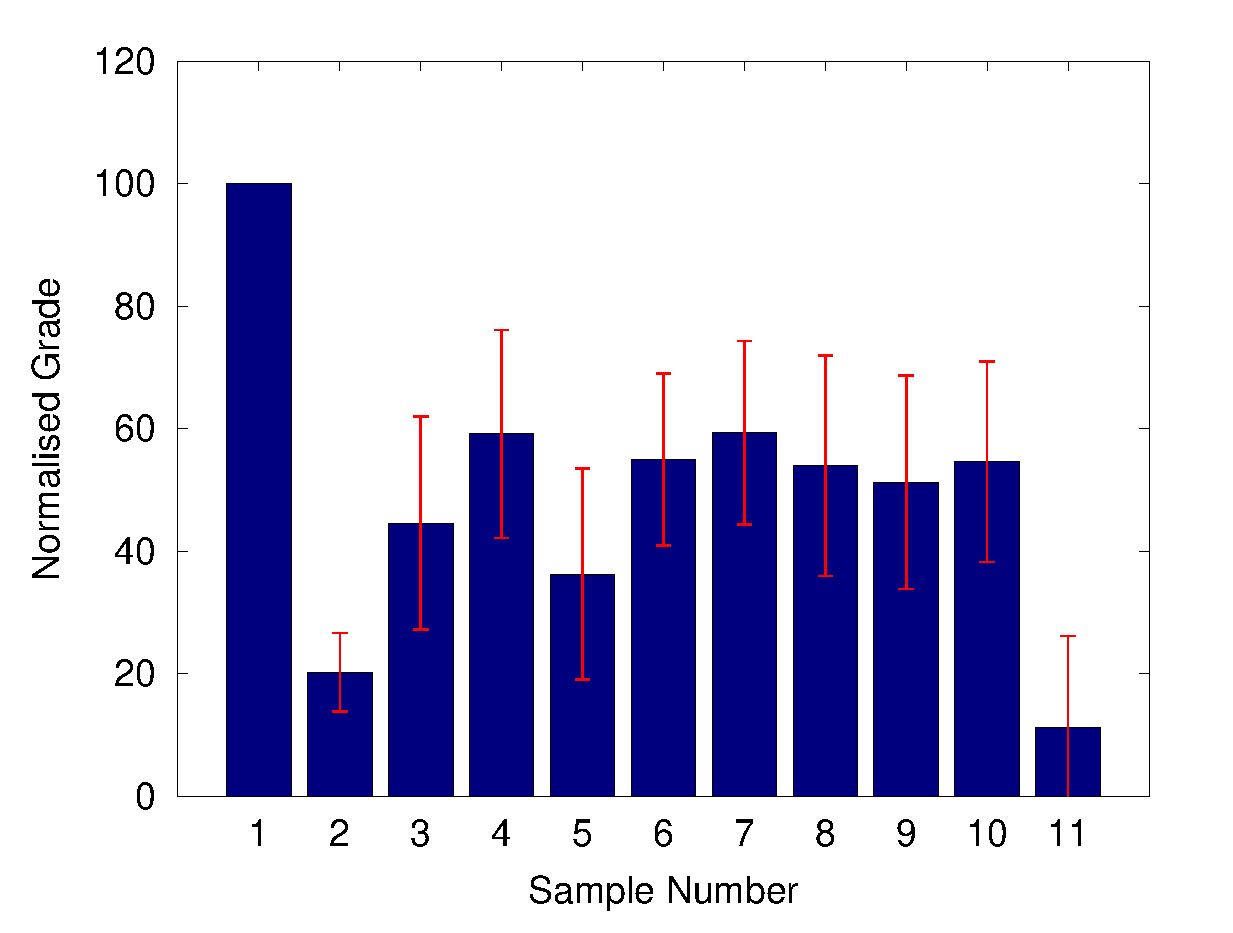
\includegraphics[width=0.45\textwidth]{chapter3/Images/CelloResults.eps}
				\label{fig:CelloResults}
			}
			\qquad
			\subfloat[Clarinet Sample]
			{
				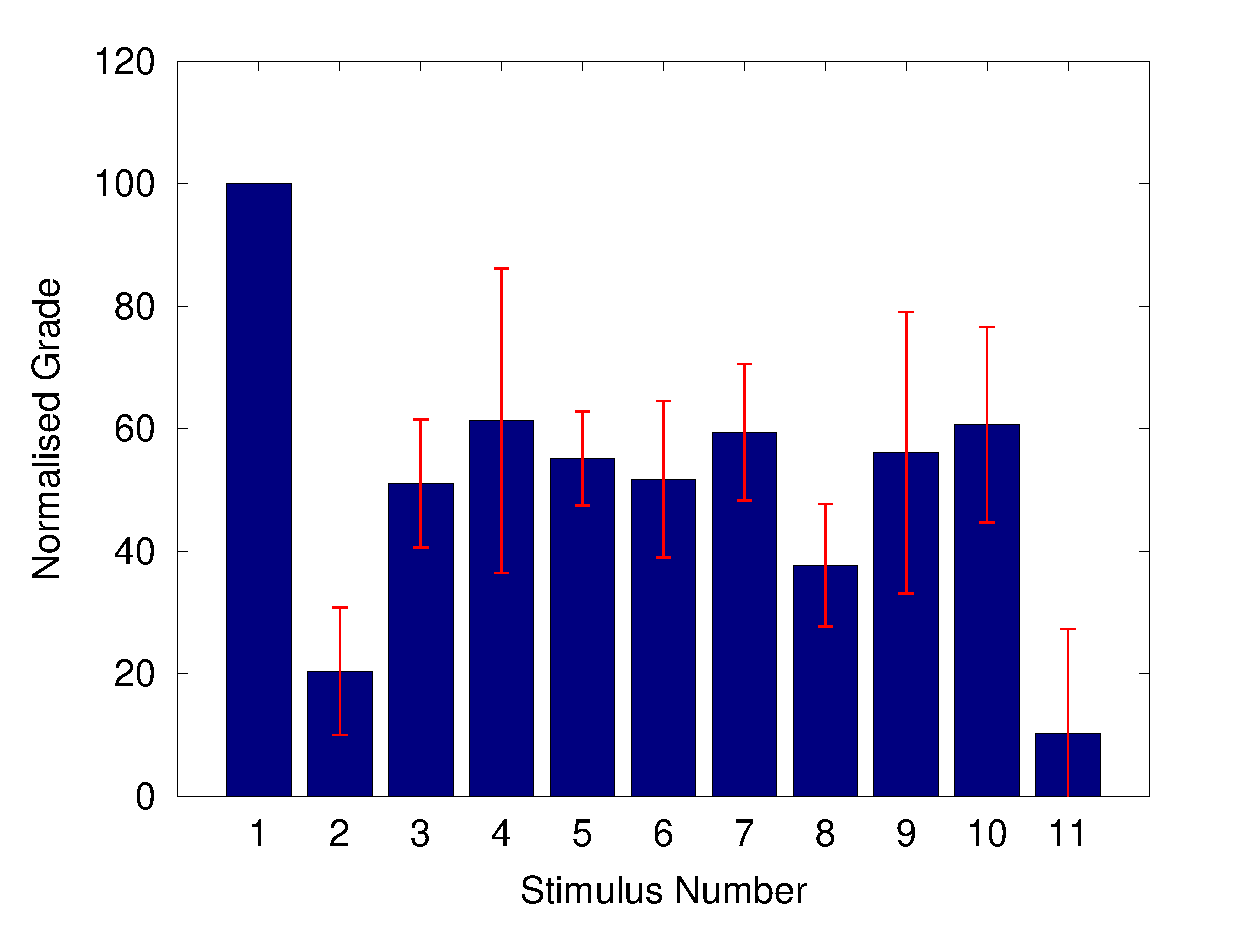
\includegraphics[width=0.45\textwidth]{chapter3/Images/ClarinetResults.eps}
				\label{fig:ClarinetResults}
			}

			\subfloat[Synthesised Sample]
			{
				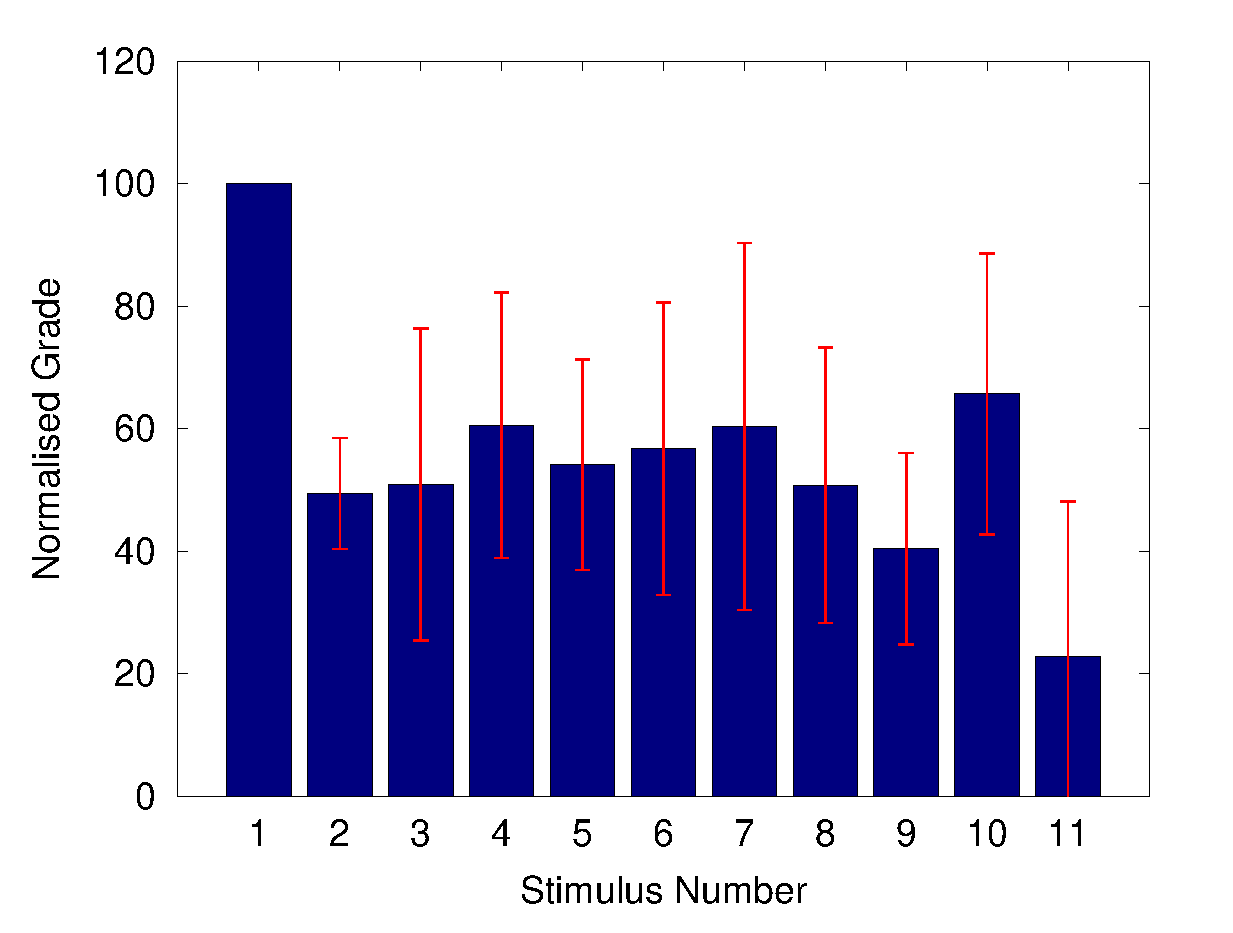
\includegraphics[width=0.45\textwidth]{chapter3/Images/SynthResults.eps}
				\label{fig:SynthResults}
			}
			\qquad
			\subfloat[Piano Sample]
			{
				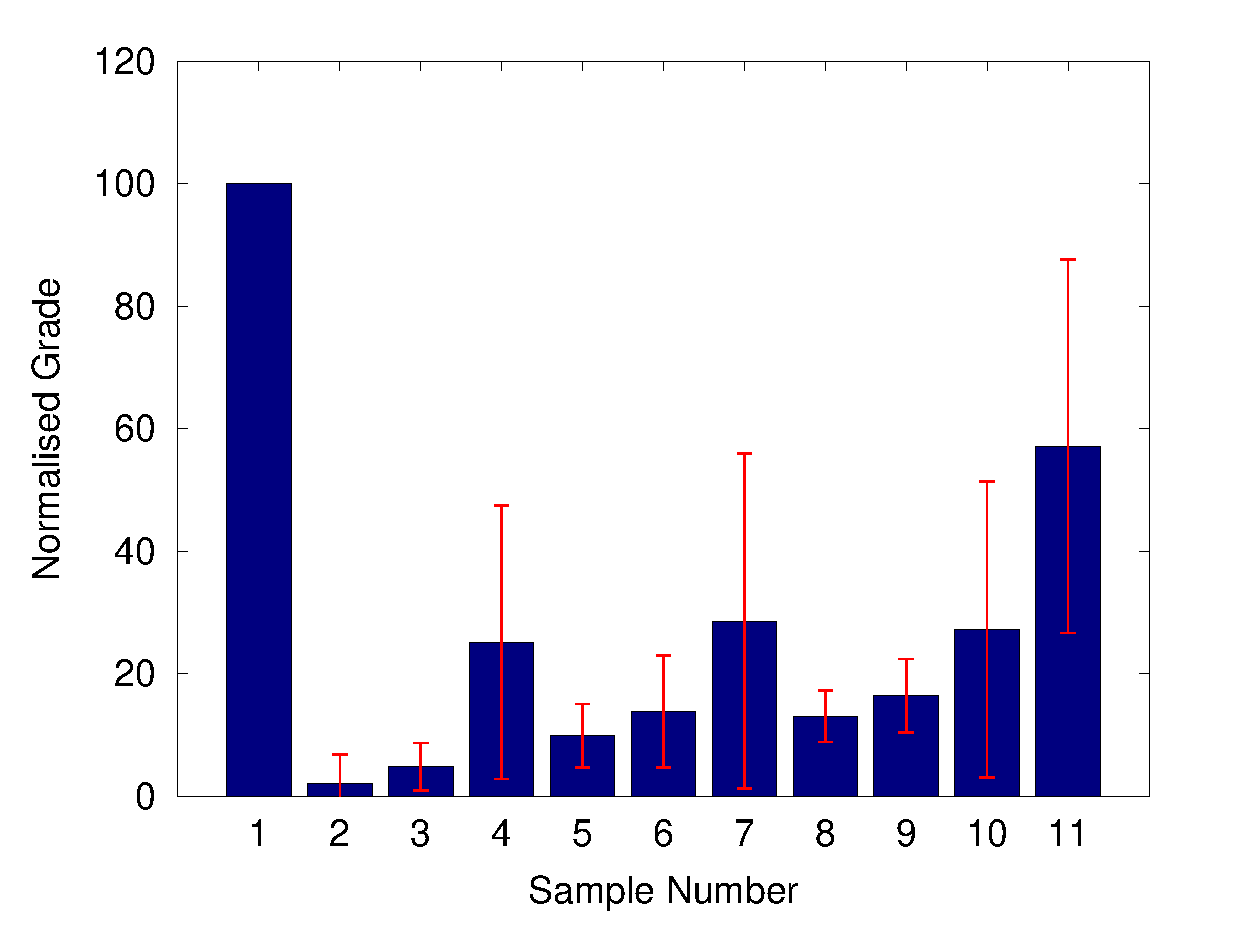
\includegraphics[width=0.45\textwidth]{chapter3/Images/PianoResults.eps}
				\label{fig:PianoResults}
			}
			\caption{Mean grades and confidence intervals for each of the stimuli.}
			\label{fig:SMCResults}
		\end{figure}

		Across all the samples there is a general increase in the perceived quality of the reproduction as the
		filter order or STFT window length is increased. With the SSBA and IAP methods increasing the filter order
		increases the level difference between the fundamental and its harmonics, better isolating the fundamental.
		This is turn reduces the levels of intermodulation distortion in the output producing a `cleaner' harmonic.
		With the synthesis method increasing the STFT window length increases the frequency resolution allowing for
		the amplitude envelope of the fundamental frequency to be measured more accurately.

		The piano sample used had very little energy at its fundamental frequency. This illustrates the problem
		discussed previously, there is not enough information in the amplitude envelope of the fundamental to
		reproduce the other harmonics. This leads to much lower grades for the reproduced signals than for any of
		the other samples. Figure \ref{fig:PianoResults} shows that the piano sample with its harmonics
		missing received a higher grade on average then any of the reconstructed samples further showing how poor
		the quality of the reconstructions is.

		The confidence intervals for the grades given to the majority of the stimuli are high. This is most likely
		due to there being too few participants in the experiment. To supplement these results each of the stimuli
		was graded with the R\sub{nonlin} metric. These results were normalised to the same range as the results
		from the listening test and are displayed in Figure \ref{fig:SMCRNonlin}.

		\begin{figure}[h!]
			\centering
			\subfloat[Cello Sample]
			{
				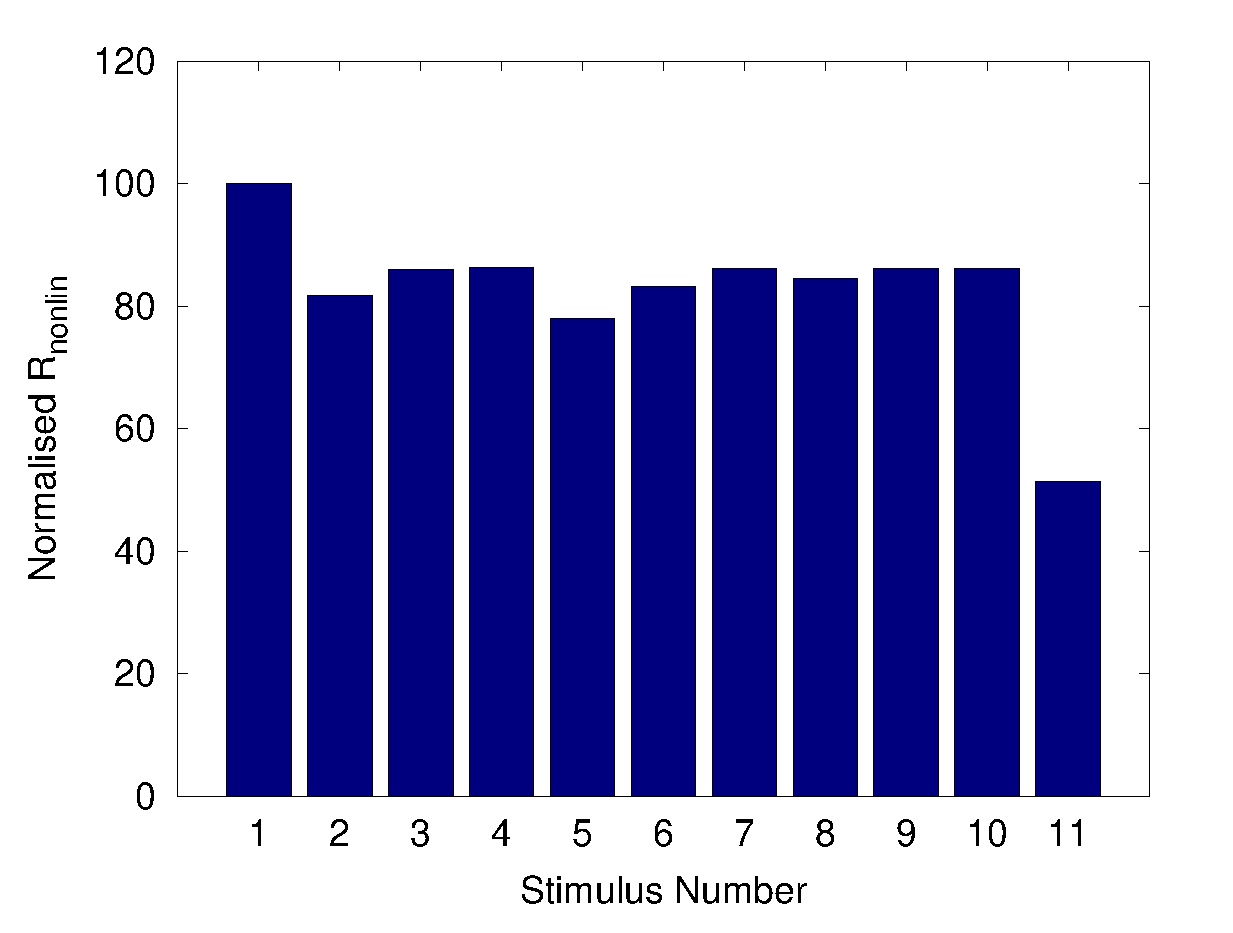
\includegraphics[width=0.45\textwidth]{chapter3/Images/CelloRNonlin.eps}
				\label{fig:CelloRNonlin}
			}
			\qquad
			\subfloat[Clarinet Sample]
			{
				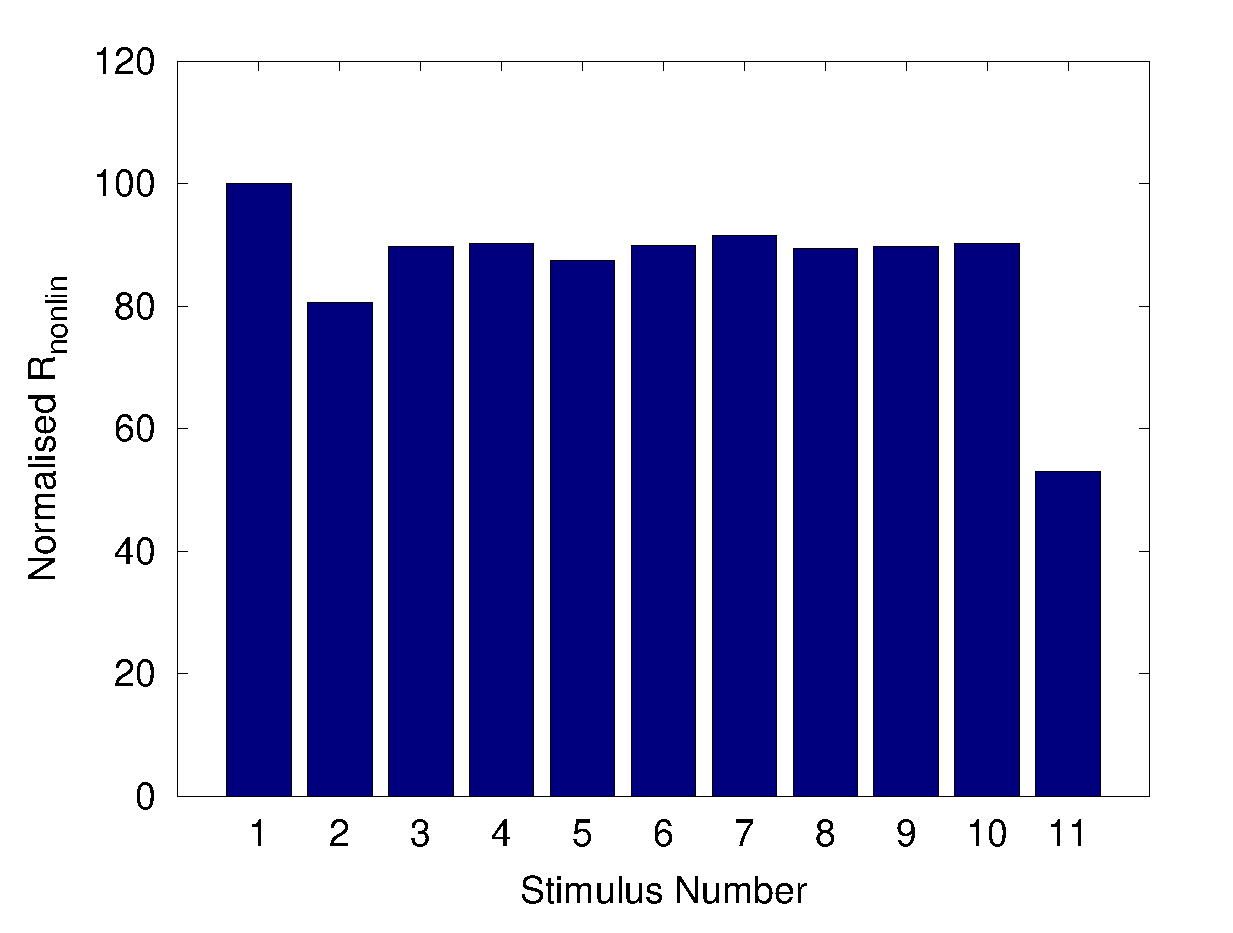
\includegraphics[width=0.45\textwidth]{chapter3/Images/ClarinetRNonlin.eps}
				\label{fig:ClarinetRNonlin}
			}

			\subfloat[Synthesised Sample]
			{
				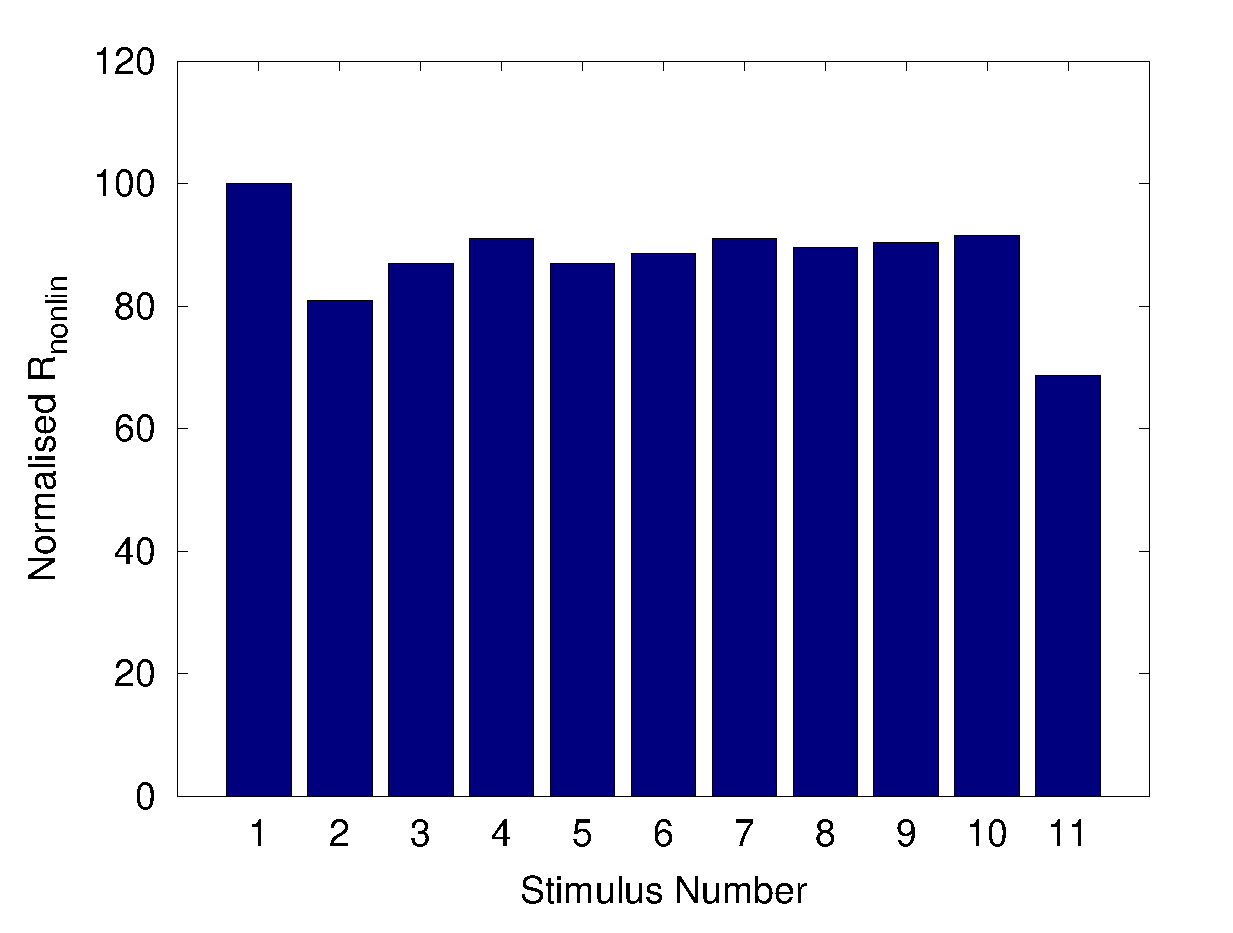
\includegraphics[width=0.45\textwidth]{chapter3/Images/SynthRNonlin.eps}
				\label{fig:SynthRNonlin}
			}
			\qquad
			\subfloat[Piano Sample]
			{
				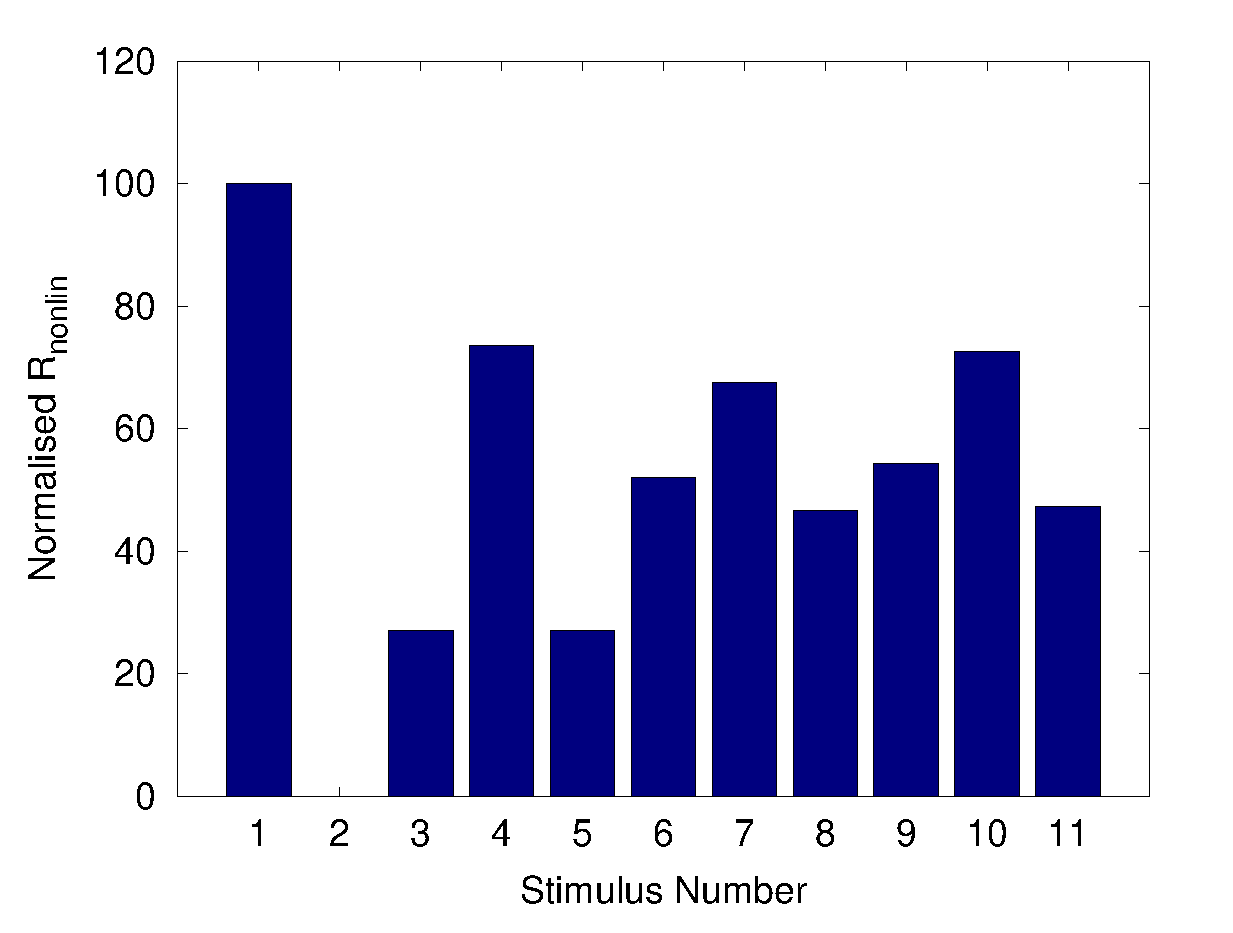
\includegraphics[width=0.45\textwidth]{chapter3/Images/PianoRNonlin.eps}
				\label{fig:PianoRNonlin}
			}
			\caption{R\sub{nonlin} values for each of the stimuli.}
			\label{fig:SMCRNonlin}
		\end{figure}

		The R\sub{nonlin} values support the correlations found in the listening test results. Using a higher order
		filter to isolate the fundamental improves the quality of the reconstruction. Figure \ref{fig:PianoRNonlin}
		again illustrates the problems which arise when the input signal has little energy at its fundamental
		frequency. Several of the reconstructions are objectively less similar to the original than the anchor
		stimulus is. 

	\subsection{Psychoacoustic Enhancement}
	\label{sec:Excitation-Enhancement}
		
		\note
		{
			Probably the most well known perceptual control effects out there. The Aural Exciter has been 
			covered by both \citet{chalupper2000aural} and \citet{shekar2013modeling}.
		}

%\section{Evaluating Excitation Methods}
%\label{sec:FeatureControl-MethodEvaluation}
%
%	\note{Homogeneity a la DAFx paper.
%	      Flexibility introduced by allowing single harmonic control a la SMC paper}
%
%	Several harmonic excitation methods were discussed in Section \ref{sec:Excitation-Methods}. When applied to the 
%	task of controlling specific audio features each of these methods has its own advantages and disadvantages.
%
%	\subsection{Homogeneity}
%	\label{sec:FeatureControl-Homogeneity}
%
%		\subsubsection*{Static Nonlinearities}		
%			As previously mentioned simple static nonlinearities are very susceptible to change in input 
%			amplitude. \citet{deman2014adaptive} counteract this issue by having the clipping threshold adapt 
%			to changes in the RMS amplitude of the input. The user is then provided with a `relative threshold' 
%			parameter on which the same setting should give similar perceptual results no matter what the input 
%			amplitude.
%
%			\note{Talk about the issues with static nonlinearities raised in \citet{enderby2012harmonic}}
%
%		\subsubsection*{Bandwidth Extension}
%			\note{Spectral mirroring, stretching and replication are all homogeneous.}
%			
%		\subsubsection*{Single Harmonic Generation}
%			Using single sideband automodulation the proportion of new frequency components in the output 
%			signal increases as the input amplitude increases. The instantaneous amplitude and phase and phase 
%			vocoder techniques are more robust in this respect.
%
%	\subsection{Flexibility}
%	\label{sec:FeatureControl-Flexibility}
%
%		\note{Flexibility is provided by individual harmonic generation \citep{enderby2013methods}}	
%
%	\subsection{Complexity}
%	\label{sec:FeatureControl-Complexity}
%		
%		\note{It is advantageous to use an algorithm that will create accurate harmonics with little analysis.
%		      Most methods don't rely on knowing the fundamental in order to generate harmonics. Spectral
%		      shifting on the other hand does.}
%
%		\note{Most of the algorithms can be easily improved through the use of a low pass filter, increasing
%	             complexity.}
